%
% Modelo para Capa final de tese de doutoramento
% do MEI.
%
% Incorpora elementos impostos pelo Regulamento de Estudos Pos-Graduados da
% Universidade de Lisboa (DR: 31/08/2017)
%
\documentclass[
 paper=A4,               % paper size --> A4 is default in Germany
    twoside=true,           % onesite or twoside printing
    openright,              % doublepage cleaning ends up right side
    parskip=full,           % spacing value / method for paragraphs
    chapterprefix=true,     % prefix for chapter marks
    11pt,                   % font size
    headings=normal,        % size of headings
    bibliography=totoc,     % include bib in toc
    listof=totoc,           % include listof entries in toc
    titlepage=on,           % own page for each title page
    captions=tableabove,    % display table captions above the float env
    draft=false,            % value for draft version
]{scrreprt}

%\DeclareOldFontCommand{\bf}{\normalfont\bfseries}
\usepackage{newstyle}
\usepackage[utf8]{inputenc}
\usepackage{amsmath,amsfonts,amssymb,amsthm,url,array}

% Quem tiver problemas com os acentos, trocar utf8 por latin1
\usepackage[portuguese,english]{babel}
\usepackage{times}
\usepackage{graphicx}
\usepackage{xspace}
\usepackage{setspace}
\usepackage[show]{chato-notes}
\usepackage[sort&compress,numbers]{natbib}
\usepackage[vlined,ruled,commentsnumbered,linesnumbered]{algorithm2e} 


% Indice remissivo
\usepackage{makeidx}
\makeindex

% Glossario
%\usepackage{glossaries}
%\makeglossary


% Links
\usepackage{hyperref}

% Package para cabecalhos
\usepackage{fancyhdr}
\usepackage{lastpage}
\usepackage{listings}
%\usepackage[subfigure]{tocloft}

\theoremstyle{definition}
\newtheorem{defn}{Definition}[]
\usepackage{tikz}
\newcommand*\circled[1]{\tikz[baseline=(char.base)]{
            \node[shape=circle,fill,inner sep=1pt] (char) {\textcolor{white}{#1}};}}

\definecolor{codegreen}{rgb}{0,0.6,0}
\definecolor{codegray}{rgb}{0.5,0.5,0.5}
\definecolor{codepurple}{rgb}{0.58,0,0.82}
\definecolor{backcolour}{rgb}{0.95,0.95,0.92}

\lstdefinestyle{mystyle}{
    backgroundcolor=\color{backcolour},
    commentstyle=\color{codegreen},
    keywordstyle=\color{blue},
    keywordstyle={[2]\color{magenta}},
    numberstyle=\tiny\color{codegray},
    stringstyle=\color{codepurple},
    basicstyle=\footnotesize,
    comment=[l]{\%},
    keywords={@relation,@attribute,@data,modifyvm, do, Vagrant, configure, id},
    morekeywords=[2]{real,integer,numeric,string,date,provider,customize,gui,v,provision, config,vm,box,ssh,insert_key,network},
    breakatwhitespace=false,
    breaklines=true,
    captionpos=b,
    keepspaces=true,
    numbers=left,
    numbersep=5pt,
    showspaces=false,
    showstringspaces=false,
    showtabs=false,
    tabsize=1
}

\lstset{style=mystyle}

\usepackage{xcolor}


\newtheorem*{validity}{Validity}{}
\newtheorem*{liveness}{Liveness}{}
\newtheorem*{security}{Compliance}{}
\newtheorem*{resilience}{Resilience}{}
\newtheorem{definition}{Definition}[]
\newtheorem{assumption}{Assumption}[]

\newcommand{\sender}{\emph{sender-SQ}\xspace}
\newcommand{\Sender}{\emph{Sender-SQ}\xspace}
\newcommand{\senders}{\emph{sender-SQs}\xspace}
\newcommand{\Senders}{\emph{Sender-SQs}\xspace}
\newcommand{\presieve}{\emph{pre-SQ}\xspace}
\newcommand{\Presieve}{\emph{Pre-SQ}\xspace}
\newcommand{\Presieves}{\emph{Pre-SQs}\xspace}
\newcommand{\presieves}{\emph{pre-SQs}\xspace}
\newcommand{\repsieve}{\emph{replica-SQ}\xspace}
\newcommand{\Repsieve}{\emph{Replica-SQ}\xspace}
\newcommand{\repsieves}{\emph{replica-SQs}\xspace}
\newcommand{\Repsieves}{\emph{Replica-SQs}\xspace}
\newcommand{\postsieve}{\emph{post-SQ}\xspace}
\newcommand{\Postsieve}{\emph{Post-SQ}\xspace}

\newcommand{\msg}{\texttt{Msg}\xspace}
\newcommand{\sn}{\emph{sn}\xspace}
\newcommand{\signature}{\emph{sgn}\xspace}
\newcommand{\mac}{\emph{mac}\xspace}
\newcommand{\senderi}{\emph{S}\xspace}
\newcommand{\sendersqi}{\emph{SQ}\xspace}
\newcommand{\presievei}{\emph{PS}\xspace}
\newcommand{\replicak}{\emph{RS}\xspace}
\newcommand{\postsievej}{\emph{PQ}\xspace}
\newcommand{\receiverj}{\emph{R}\xspace}
\newcommand{\privkey}{\emph{prk}\xspace}
\newcommand{\pubkey}{\emph{puk}\xspace}
\newcommand{\sharedkey}{\emph{shk}\xspace}


\newcommand{\system}{\textsc{Lazarus}\xspace}
\newcommand{\sieveq}{\textsc{SieveQ}\xspace}
\newcommand{\controller}{\textsc{Baton}\xspace}
\newcommand{\fetcher}{\emph{Data manager}\xspace}
\newcommand{\manager}{\emph{Deploy manager}\xspace}
\newcommand{\risk}{\emph{Risk manager}\xspace}

\newcommand{\block}{\emph{Diversity block}\xspace}
\newcommand{\blocks}{\emph{Diversity blocks}\xspace}
\newcommand{\replica}{\emph{replica}\xspace}
\newcommand{\replicas}{\emph{replicas}\xspace}
\newcommand{\configuration}{\emph{System configuration}\xspace}
\newcommand{\configurations}{\emph{System configurations}\xspace}
\newcommand{\configurationClean}{System configuration}


\newcommand{\systemformula}{risk\xspace}
\newcommand{\pairformula}{common\xspace}
\newcommand{\vulnerabilityformula}{score\xspace}


\SetKwData{RS}{\texttt{POOL}}
\SetKwData{ES}{\texttt{CONFIG}}
\SetKwData{PS}{\texttt{CANDIDATES}}
\SetKwData{RM}{\texttt{REMOVABLES}}
\SetKwData{QS}{\texttt{QUARANTINE}}
\SetKwData{MAX}{\texttt{MAXIMALS}}
\SetKwData{N}{\texttt{N}}
\SetKwData{r}{\texttt{r}}
\SetKwData{K}{\texttt{K}}
\SetKwData{toRemove}{\texttt{toRemove}}
\SetKwFunction{Rand}{rand}
\SetKwFunction{Size}{size}
\SetKwFunction{Remove}{rm}
\SetKwFunction{Risk}{risk}
\SetKwFunction{Common}{common}
\SetKwFunction{Older}{older}
\SetKwFunction{healing}{init\_healing}
\SetKwFunction{Inc}{increment}
\SetKwFunction{Dec}{decrement}
\SetKwProg{Fn}{Function}{}{}

\fancyhf{} %
\lhead{\nouppercase {\leftmark}} %
\rhead{\nouppercase {\bf \thepage}}
\renewcommand{\headrulewidth}{0.1pt}

% Comando para inserir pagina em branco (inserida na numeracao, mas sem
% numero impresso) para quando e' preciso obrigar um capitulo a comecar
% do lado direito (pagina impar)
\newcommand{\LIMPA}{
\newpage
\mbox{}
\thispagestyle{empty}
}

% Igual, mas insere pagina com numero impresso (normalmente nao se usa)
\newcommand{\LIMPAC}{
\newpage
\mbox{}
\thispagestyle{plain}
}

%
% ALTERAR AQUI AS INFORMACOES RELATIVAS AO PROJECTO
%
\newcommand{\TITULO}{DIVERSE INTRUSION-TOLERANT SYSTEMS}
\newcommand{\Autor}{Miguel Garcia Tavares Henriques}
\newcommand{\AutorNumAluno}{35054}

%Orientador e CoOrientador *sem* titulos (e.g. Prof. Doutor)
\newcommand{\Orientador}{Alysson Neves Bessani}
\newcommand{\CoOrientador}{Nuno Fuentecilla Maia Ferreira Neves} %se nao se aplicar, nao importa o que aqui esteja

%Se aplicavel, o supervisor pode ter um titulo (Dr., Eng.) colocado aqui
\newcommand{\SupervisorInstituicao}{Nome Completo do Supervisor}  %se nao se aplicar, nao importa o que aqui esteja

\newcommand{\AnoLectivo}{2017/2018}
\newcommand{\Ano}{\Large{2018}}

% Comentar/descomentar conforme conveniente
\newcommand{\TIPO}{DISSERTA\c{C}\~{A}O }
%\newcommand{\TIPO}{TRABALHO DE PROJETO }

% Comentar/descomentar conforme conveniente
%\newcommand{\MESTRADO}{MESTRADO EM -- PREENCHER --}
\newcommand{\DOUTORAMENTO}{Doutoramento em Inform\'{a}tica}

% Comentar/descomentar conforme conveniente
%\newcommand{\IdiomaTese}{\selectlanguage{portuguese}}
\newcommand{\IdiomaTese}{\selectlanguage{english}}

% Comentar/descomentar conforme conveniente
\newcommand{\Especialidade}{}

\newcommand{\Cabecalho}{
\vspace{1cm}\normalfont\normalfont
\vfill
\textsc{\normalsize\uppercase{Universidade de Lisboa}}\\
\normalsize\uppercase{Faculdade de Ci\^{e}ncias}\\
\vspace{1cm}

\includegraphics[scale=.45]{pic/logo_fcul_vertical.png}\\
}

\usepackage{ifpdf}
\ifpdf
\pdfinfo {
	/Author (\Autor)
	/Title (\TITULO)
	/Subject (\DOUTORAMENTO)
	/Keywords ()
	/CreationDate (D:20081112151803)
}
\fi

%\usepackage[dvips]{geometry}
%\geometry{a4paper=true,portrait=true,left=3cm,right=3cm,top=2.5cm,bottom=3.5cm}

\title{\TITULO}
\author{\Autor}
%\date{\today}

\usepackage{glossaries}
\makeglossaries

\begin{document}
\selectlanguage{english}
\pagestyle{empty}

% Primeira capa
% 
%
\begin{center}

\Cabecalho

\vspace{2.0cm}
\vfill
\IdiomaTese
\Large{\bf \TITULO}\\
\vspace{2cm}
\vfill

\large{\bf{\DOUTORAMENTO}}\\
%\normalsize{\Especialidade}\\
\vspace{2.0cm}
\vfill
\Large{\bf \Autor}\\
\vspace{1,8 cm}
\vfill
\large{Tese orientada por:}\\
%\normalsize{Trabalho de projeto orientado por:}\\
\large{Prof. Doutor \Orientador} \\
% DESCOMENTAR a linha relevante (se alguma), removendo o % no inicio
e co-orientada pelo Prof. Doutor \CoOrientador \\
\vspace{1 cm}
\vfill

\normalsize{Documento especialmente elaborado para a obten\c{c}\~{a}o do grau de doutor}
\vspace{0.5cm}
\vfill
\Ano
\end{center}
\newpage
\mbox{}
\newpage

%
% Segunda capa
%

\begin{center}

\Cabecalho

\vspace{0.5cm}
\vfill
\IdiomaTese
\Large{\bf \TITULO}\\
\selectlanguage{portuguese}
\vspace{1cm}
\vfill

\large{\bf{\DOUTORAMENTO}}\\
%\normalsize{\Especialidade }\\
\vspace{1cm}
\vfill
\Large{\bf \Autor}\\
\vspace{.5 cm}
\vfill
\large{Tese orientada por:}\\
%\normalsize{Trabalho de projeto orientado por:}\\
\large{Prof. Doutor \Orientador} \\
% DESCOMENTAR a linha relevante (se alguma), removendo o % no inicio
e pelo Prof. Doutor \CoOrientador \\
\vspace{.5 cm}
\vfill

\begin{flushleft}  
\large{J\'{u}ri}
\vfill
\setlength{\leftskip}{0.5cm}
\normalsize{Presidente:}
\begin{itemize}
\setlength\itemsep{-0.5 em}
\item{Nome do Presidente}
\end{itemize}
\normalsize{Vogais:}
\begin{itemize}
\setlength\itemsep{-0.5 em}
\item{Nome do Vogal}
\item{Nome do Vogal}
\item{Nome do Vogal}
\item{Nome do Vogal}
\end{itemize}
\setlength{\leftskip}{0cm}
\end{flushleft}
\vspace{0.0cm}
\vfill

\normalsize{Documento especialmente elaborado para a obten\c{c}\~{a}o do grau de doutor\par}
\vspace{0.0cm}
\normalsize{Este trabalho foi financiado pela Funda\c{c}\~{a}o para a Ci\^{e}ncia e Tecnologia (FCT) atrav\'{e}s da Bolsa Individual de Doutormento SFRH/BD/84375/2012 e atrav\'{e}s dos projectos da Comiss\~{a}o Europeia FP7-257475 (MASSIF) e H2020-700692 (DiSIEM).}
\vspace{0.cm}
\vfill
\Ano
\end{center}
\newpage
\mbox{}
\newpage
% Fim da capa
% ----------------------------------------------------------------------

% This work was supported by Fundação para a Ciência e a Tecnologia (FCT), through Multiannual
%Funding to the LaSIGE research unit and the Individual Doctoral Grant SFRH/BD/84375/2012.
\setcounter{page}{1}
\pagenumbering{roman}

\addcontentsline {toc} {chapter} {Acks}
\pagestyle{plain}

\vspace*{2cm}
\selectlanguage{portuguese}
\chapter*{Agradecimentos}

%\begin{center}
%\selectlanguage{portuguese}
%\Large \bf Agradecimentos
%\selectlanguage{english}

Este documento encerra todo trabalho feito ao longo de alguns anos desde o mestrado até agora. 
Durante estes anos tive a sorte de trabalhar com dois investigadores de grande qualidade, os meus orientadores Professor Alysson Bessani e Professor Nuno Neves.
Devo-lhes um sincero obrigado por todos os ensinamentos e orientações que me transmitiram. 
Cada um da sua forma contribuiram para o meu crescimento como pessoa e investigador. 

A todos os meus colegas e amigos do LASIGE e DI, aos que vieram e foram e aos que vieram  e ficam, em todas as fases do doutoramente tive rodeado de boa gente. Em especial um agradecimento ao Tiago, Ibéria, Vavala, Eduardo, João, Fernando, André e ao Vinicius. A vossa amizade, companheirismo, compreensão, inter-ajuda e motivação foram essenciais nesta fase.  

A todos os meus amigos fora deste "universo" que de uma forma ou de outra contribuiram para este tese. 
Mesmo sem compreenderem bem o que eu fazia devo-lhes a boa disposição e animo. 
O prêmio de paciência vai para o Bruno, Paulo e Gonçalo.


Sem a minha familia seria impossível chegar ao fim desta maratona. 
Aos de casa e aos que escolhi para serem parte da minha familia.
Em especial à minha mãe, aos meus irmãos Diogo e Joana, à Vanessa e à Ana por serem incansáveis e se hoje sou mais forte é porque tive o vosso apoio.
Obrigado e espero que tenham orgulho em mim. 



%\Large \bf Acknowledgments
%\end{center}
%\vspace*{1cm} \setlength{\baselineskip}{0.6cm}



\LIMPA
\LIMPA

\vfill

%\selectlanguage{portuguese}

\begin{flushright}\textit{Para a minha avó.}\end{flushright}

\LIMPA


\addcontentsline {toc} {chapter} {Abstract (PT)}
% Pagina do resumo em portugues
%\pagestyle{empty}

% ----------------------------------------------------------------------
% P�gina do resumo em Portugu�s:
\selectlanguage{portuguese}
\chapter*{Resumo}
\label{chapter:abstract_pt}
\vspace*{-10mm}


\vfill

\begin{flushleft}
\textbf{Palavras-chave:}
Diversidade, Vulnerabilidades, Sistemas Operativos, Toler\^{a}ncia a Intrus\~{o}es, Recuper\c{c}\~{a}o Proactiva.
\end{flushleft}

\LIMPA
% Fim da p�gina do resumo em Portugu�s
% ----------------------------------------------------------------------


\addcontentsline {toc} {chapter} {Abstract (EN)}
% Pagina do resumo em ingles
% ----------------------------------------------------------------------
% P�gina do resumo em Ingl�s:
% 300 palavras
\selectlanguage{english}
%\vspace*{2cm}
%\begin{center}
%\Large \bf Abstract
%\end{center}
%\vspace*{1cm} \setlength{\baselineskip}{0.6cm}
\chapter*{Abstract}
\label{chapter:abstract_en}
\vspace*{-10mm}

Over the past 20 years, there have been indisputable advances on the development of Byzantine Fault-Tolerant (BFT) replicated systems. 
These systems keep operational safety as long as at most $f$ out of $n$ replicas fail simultaneously. 
Therefore, in order to maintain correctness it is assumed that replicas do not suffer from common mode failures, or in other words that replicas fail independently. 
In an adversarial setting, this requires that replicas do not include similar vulnerabilities, or otherwise a single exploit could be employed to compromise a significant part of the system. 
The thesis investigates how this assumption can be substantiated in practice by exploring diversity when managing the configurations of replicas.

The thesis begins with an analysis of a large dataset of vulnerability information to get evidence that diversity can contribute to failure independence. 
In particular, we used the data from a vulnerability database to devise strategies for building groups of $n$ replicas with different Operating Systems (OS). 
Our results demonstrate that it is possible to create dependable configurations of OSes, which do not share vulnerabilities over reasonable periods of time (i.e., a few years).

Then, the thesis proposes a new design for a firewall-like service that protects and regulates the access to critical systems, and that could benefit from our diversity management approach. 
The solution provides fault and intrusion tolerance by implementing an architecture based on two filtering layers, enabling efficient removal of invalid messages at early stages in order to decrease the costs associated with BFT replication in the later stages.

The thesis also presents a novel solution for managing diverse replicas. 
It collects and processes data from several data sources to continuously compute a risk metric. 
Once the risk increases, the solution replaces a potentially vulnerable replica by another one, 
trying to maximize the failure independence of the replicated service. 
Then, the replaced replica is put on quarantine and updated with the available patches, to be prepared for later re-use. 
We devised various experiments that show the dependability gains and performance impact of our prototype, including key benchmarks and three BFT applications (a key-value store, our firewall-like service, and a blockchain). 

%This thesis addresses the problem of building dependable Byzantine fault-tolerant (BFT) systems through diversity. 
%Although the indisputable contributions of many works from the BFT research community, diversity management still is a long-standing open problem of this area. 
%BFT safety holds under the strict assumption that only $f$ out $n$ replicas fail \emph{simultaneously}.
%Therefore, it is assumed that replicas fail independently (e.g., they do not share vulnerabilities).
%Otherwise, the amount of effort to compromise $f$ replicas would be the same as to compromise $f+1$, becoming easier to break the BFT safety.


%The thesis begins with an analysis (that is in some part prior to this thesis) on security data.
%This analysis shows evidence to support failure independence among BFT replicas.
%In particular, we used a vulnerability database to build sets of $n$ replicas with different Operating Systems (OS).
%Based on these results, it is possible to create dependable configurations of OSes of BFT systems. 


%Nevertheless, we have identified some limitations on the previous analysis. 
%These were mainly due to missing data that would provide inaccurate results.
%Therefore, we designed a more advanced solution to manage the diversity of any BFT system. 
%We developed a solution that considers several (free) security data sources.
%This data, feeds a novel metric that is used to make decisions on diversity sets minimizing the common vulnerabilities.
%We developed a methodology to address off-the-shelf diversity in general. 
%However, here we focused on OSes as there resides the replica's major code complexity.
%Moreover, we extended this contribution in a more practical way and developed a prototype that enables automatic management of BFT replicas' diversity.
%Hence, we reduce the complexity inherent from dealing with diverse software in replicated systems. 

%We devised a few experiments that show the dependability gains of using an advanced diversity selection and the impact of using different OSes in a few BFT applications (one of them is a BFT firewall-like that is part of the contributions of this thesis).
%Nevertheless, implementation decisions made us pay an additional cost on the performance to achieve such results on dependability.

\vfill

\begin{flushleft}
\textbf{Keywords:}
Diversity, Vulnerabilities, Operating Systems, Intrusion Tolerance, Rejuvenations.
\end{flushleft}

%\LIMPA

% Fim da p�gina do resumo em Ingl�s.
% ----------------------------------------------------------------------




\tableofcontents

\LIMPA

%Lista de figuras
\listoffigures

\addcontentsline {toc} {chapter} {List of Figures}
\newpage
\thispagestyle{empty}
\mbox{}
\newpage

%Lista de tabelas
\listoftables

\addcontentsline {toc} {chapter} {List of Tables}
\newpage
\thispagestyle{empty} \mbox{}
\newpage

% ----------------------------------------------------------------------
% Inicio conteudo
\pagestyle{fancy}
\cleardoublepage

\setcounter{page}{1}
\pagenumbering{arabic}
\chapter{Introduction}
\label{chap:introduction}

\section{Context and Motivation}
\gls{bft}\footnote{In this thesis we interchange Byzantine fault tolerance (subject) with Byzantine fault-tolerant (adjective) using the same acronym BFT for both.} is a well-established area of research that aims to guarantee safety on replicated systems even in the presence of some (Byzantine) faulty nodes.
In a nutshell, \gls{bft} protocols guarantee that replicas agree on the order of the message execution, and thus, the replicas work as a replicated state machine.
The overall \gls{bft} safety holds even if a subpart of replicas, typically $f$ out of $n$, is faulty, leaving a sufficient number of correct nodes that execute correctly.
Although not explicit, this assumption leverages on the strict condition that nodes (must) fail independently.
Otherwise, compromising $f$ replicas is virtually the same as compromising $f+1$.


\gls{bft} was first proposed in 1982 by Lamport~\etal{}~\cite{Lamport:1982}, but it only as awaken the distributed systems research community to its relevancy in 1999 due to Castro and Liskov's Practical \gls{bft}~\cite{Castro:1999}. 
In the last twenty years of active research on \gls{bft} replication, there were made great advances on the performance (e.g.,~\cite{Kotla:2010,Aublin:2015,Behl:2015}), use of resources (e.g.,~\cite{Yin:2003,Wood:2011,Veronese:2013,Liu:2016,Behl:2017}), and robustness (e.g.,~\cite{Amir:2011,Bessani:2014,Clement:2009b}) of \gls{bft} systems.
However, \gls{bft} in general and these works in particular, assume, either implicitly or explicitly, that the replica nodes fail independently. 
This assumption extends the fault threshold as it considers that it takes more time/effort to compromise replicas that do not share vulnerabilities.
Nevertheless, a few works rely on some orthogonal mechanisms (e.g.,~\cite{Roeder:2010,Chen:1995}) to avoid these common weaknesses, or rule out the possibility of malicious failures from their system models.
Moreover, a few works have implemented and experimented with such mechanisms (e.g.,~\cite{Rodrigues:2001,Roeder:2010,Amir:2011}), but in a very limited way.


In practice, a few dependable applications take advantage of diversity mechanism. 
Nevertheless, in these cases, diversity is applied \emph{intuitively}.
For example, in avionics engineering, a few aircraft solutions embrace the diversity of components to avoid accidental failures~\cite{Yeh:2004}.
Moreover, in 2014, the U.S. Navy developed the Resilient Hull, Mechanical, and Electrical Security (\textsc{Rhimes}), it introduces diversity through a \emph{slightly different implementation} for each programmable logic controller~\cite{rhimes}.
Another example of a critical system that naturally adopted diversity are the \gls{dns} root servers. 
According to Lars-Johan Liman (the technical lead of one of the \gls{dns} root servers),\footnote{https://www.netnod.se/dns/dns-root-server-faq} each operator has its own configurations, as ``\emph{it allows for great operational diversity. That means, for example, that a single software or firmware bug cannot bring down the entire system}.''
\textbf{FIX THIS} On the contrary, the growing blockchain technology implements \gls{bft} in a large and dispersed network.
The proof-of-work~\cite{} solutions do not need a strictly bounded fault threshold, as their threshold is bounded by 51\% of the network is correct.


Despite the adoption of (naive) diversity in practical systems, other variables must be considered to make systems dependable and secure.
For example, even considering an initial set of $n$ diverse replicas, long-running services need to be cleaned from possible failures and intrusions.
A few works on the proactive recovery of \gls{bft} systems~\cite{Castro:2002,Sousa:2010,Roeder:2010,Platania:2014,Distler:2011} periodically restart their replicas to clean undetected faulty states introduced by a stealth attacker. 
However, these works (i) assume replicas failure independence, (ii) do not provide proof to support their diversity decisions or (iii) use limited solutions (e.g., memory randomization).
Therefore, unless careful selection of diversity is introduced during recoveries, the replicas do not change, thus keeping the same vulnerabilities.


Finally and despite the already established maturity of \gls{bft} solutions, no one debated how to apply diversity in a dependable (i.e., which software configurations are more dependable) and when should these configurations be changed (e.g., recovering replicas with different software).

\section{Objectives and Contributions}

In the past, several researchers developed and improved techniques to make intrusion tolerance a cornerstone of security and dependability.
Nevertheless, a few problems were left open and still lack effective answers.
This thesis aims to push forward intrusion tolerance to more accurate and practical grounds.
The main contributions of this thesis are summarized into the following points, along with the related publications.


\subsection{Evidence for Implementing Diversity}% Diversity Study on Off-the-Shelf Operating Systems}


The results achieved during the MSc thesis encouraged us to extend the work on the diversity of \gls{ots} \glspl{os}~\cite{Garcia:2012}.
This first step towards the design and development of dependable \gls{bft} systems is to assess how accurate were the implicit or explicit assumptions on diversity (e.g.,~\cite{Abd-El-Malek:2005,Bessani:2008,Castro:2002,Castro:2003,Clement:2009,Correia:2004,Kapitza:2012,Kotla:2010,Moniz:2011,Yin:2003}).
In that previous work, we studied the vulnerability data from the \gls{nvd}~\cite{nvd} the most complete vulnerability database available to answer, with arguments to support, to the question:
\emph{What are the dependability gains from using diverse \glspl{os} on a replicated  intrusion-tolerant system?} 
Nevertheless, we have made some extensions to that work, which are presented in this thesis.
In particular, we devised three manual strategies for selecting diverse software components to minimize the incidence of common vulnerabilities in replicated systems.
Moreover, we observed that using different \gls{os} releases of the same \gls{os} is enough to warrant its adoption as a more straightforward, less complicated, more manageable configuration for replicated systems.
The described contributions (together with the ones published during the MSc~\cite{Garcia:2012}) are reported in the following publication:

\begin{enumerate}
\item[1.] \textbf{Analysis of Operating System Diversity for Intrusion Tolerance}, Miguel Garcia, Alysson Bessani, Ilir Gashi Nuno Neves, and Rafael Obelheiro, in \emph{Software: Practice and Experience, 2014}~\cite{Garcia:2014}.
\end{enumerate}



\subsection{Applying Diversity on BFT Systems}
In our first attempt to validate diversity, we presented substantial evidence to claim that using different \glspl{os} guarantees failure independence to some extent.
However, this preliminary analysis suffer from some limitations as other works using \gls{nvd} database (e.g.,~\cite{Gorbenko:2011,Han:2009,Frei:2010,Shahzad:2012,Bozorgi:2010,Allodi:2014,Gorbenko:2017}).
It is possible to find vulnerabilities in \gls{nvd} that are not reported to all affected \glspl{os}.
We have found these missing vulnerabilities reported on other sources (e.g., the vendors' security advisories).
Therefore, some of the results of \gls{nvd}-based studies may provide less accurate conclusions about selecting different software based on common vulnerabilities.
Moreover, \gls{nvd} lacks from some relevant data concerning exploits and patches that are relevant when considering vulnerabilities life-cycle.
An alternative way to \gls{ots} diversity is to generate diversity through automatic mechanisms (e.g.,~\cite{Roeder:2010,Amir:2011}).
However, these mechanisms lack of evidence to claim that these techniques create real vulnerability independence~\cite{Snow:2013,Bittau:2014}. 
Finally, the existent systems that implement time-triggered recoveries assume that it takes the same time/effort to compromise each replica, by assuming that vulnerabilities are all the same. 
This assumption is unrealistic, especially when the replicas' diversity is considered~\cite{Nayak:2014}. 
Therefore, tailored methods are required to evaluate the risk of a replicated system becoming vulnerable (i.e., $f+1$ replicas suffer from the same weaknesses).


In this thesis, we address these problems from both a theoretical and practical perspective.
We address the problems of \emph{finding evidence for supporting diversity}, \emph{manage diversity in a dependable way}, and \emph{support diversity practical mechanisms} in the thesis main contribution.
First, suppress the limitations of \gls{nvd} using clustering techniques, that group similar vulnerabilities, which potentially can be affected by (variations of) the same exploit.
Moreover, we add additional \gls{osint} data sources to build a complete knowledge base about the possible vulnerabilities, exploits, and patches related to the systems of interest. 
The clusters and the collected data are used to assess the risk of a \gls{bft} system becoming compromised by the existence of common vulnerabilities.
Once the risk increases, the system replaces the potentially vulnerable replica by another one, to maximize the failure independence of the replicated service.
The solution continuously collects data from the online sources and monitors the risk of the \gls{bft} in such a way that removes the human from the loop.

We have implemented these contributions in \system, and it is the first system that automatically changes the attack surface of a \gls{bft} system in a dependable way.
\system continuously collects security data from several \gls{osint} feeds to build a vulnerability knowledge base.
This data is used to create clusters of similar vulnerabilities.
These clusters and other collected attributes are used to analyze the risk of the \gls{bft} system becoming compromised. 
Once the risk increases, \system replaces the potentially vulnerable replica by another one, trying to maximize the failure independence. 
The replica's replacement is made automatically, while a new replica is deployed in the \gls{bft} group, the replaced node is put on quarantine and updated with the available patches, to be re-used later.
These mechanisms were implemented to be fully automated and transparent to \gls{bft} systems.
Moreover, the current implementation of \system manages 17 \gls{os} versions, supporting the \gls{bft} replication of a set of representative applications.
The replicas run in \glspl{vm}, allowing provisioning mechanisms to configure them. 
We conducted two sets of experiments: The first one demonstrates that \system risk management can prevent a group of replicas from sharing vulnerabilities over time; 
The second one, reveals the potential negative impact that virtualization and diversity can have on performance. 
In this experiment, we evaluated \system with three \gls{bft} use case applications: (1) a Key-Value Store application, (2) \sieveq an application-like firewall (this contribution is presented in the next section), and (3) a \gls{bft} ordering service for Hyperledger Fabric a blockchain application.
The overall results show that if naive configurations are avoided, \gls{bft} applications in diverse configurations can perform close to our homogeneous bare metal setup.

The contributions of this work resulted in the following publications:

\begin{enumerate}

\item[2.] \textbf{\textsc{Diversys}: DIVErse Rejuvenation SYStem}, Miguel Garcia, Nuno Neves, and  Alysson Bessani in the \emph{Simp\'{o}sio Nacional de Inform\'{a}tica (INFORUM), 2012~\cite{Garcia:2012b}}.


\item[3.] \textbf{Towards an Execution Environment for Intrusion-Tolerant Systems}, Miguel Garcia, Alysson Bessani, and Nuno Neves, Poster session in the \emph{European Conference on Computer Systems (EuroSys), 2016}~\cite{Garcia:2016b}.


\item[4.] \textbf{\system: Automatic Management of Diversity in BFT Systems}, Miguel Garcia, Alysson Bessani, and Nuno Neves -- \emph{Submitted for publication}.

\end{enumerate}


\subsection{BFT Multi-layer Resiliency} 
\system implements mechanisms that provide security and dependability for replicated systems.
However, not all systems need to be \gls{bft}-replicated nor managed with such advanced mechanisms. 
Some of the most critical applications that can benefit from such management are firewalls.
Firewalls are used as the primary protection against external threats, controlling the traffic that flows in and out of a network. 
Typically, they decide if a packet should go through (or be dropped) based on the analysis of its contents. 
Most generic firewall solutions suffer from two inherent problems: 
First, they have vulnerabilities as any other system, and as a consequence, they can also be the target of advanced attacks. 
For example, the \gls{nvd}~\cite{nvd} shows that there have been many security issues in commonly used firewalls. 
\gls{nvd}'s reports present the following numbers of security issues between 2010 and 2018:\footnote{To the date of Jul 12$^{th}$ 2018.} 205 for the Cisco Adaptive Security Appliance; 123 in Juniper Networks solutions; and 50 related to iptables/netfilter. 
Common protection solutions often have been the target of malicious actions as part of a wider scale attack (e.g., anti-virus software~\cite{Chauhan:2011}, \gls{ids}~\cite{Anderson:2001} or firewalls~\cite{Kamara:2003,Surisetty:2010,cisco1,cisco2}).
Second, firewalls are typically a single point of failure, which means that when they crash, the ability of the protected system to communicate may be compromised, at least momentarily.
Therefore, ensuring the correct operation of the firewall under a wide range of failure scenarios becomes imperative.


This last contribution addresses the previously described problems with a new protection system, called \sieveq.
This system mixes the firewall paradigm with a message queue service.
In the last decade, several significant advances occurred in the development of intrusion-tolerant systems.
However, to the best of our knowledge, very few works proposed intrusion-tolerant protection devices, such as firewalls.
Performance reasons might explain this, as \gls{bft} replication protocols are usually associated with significant overheads and limited scalability.
Additionally, achieving complete transparency to the rest of the system can be challenging to reconcile with the objective of having fast message filtering under attack.
In \sieveq, we explore a different design for replicated protection devices, where we trade some transparency on senders and receivers for a more efficient and resilient firewall solution.
In particular, we propose an architecture in which critical services and devices can only be accessed through a message queue and implement the application-level filtering in this queue.
It is assumed that these services have a limited number of senders, which can be appropriately configured to ensure that only they are authorized to communicate through \sieveq.
The solution has a fault- and intrusion-tolerant architecture that applies filtering operations in two stages acting like a sieve.
The first stage, called \emph{pre-filtering}, performs lightweight checks, making it efficient to detect and discard malicious messages from external adversaries.
In particular, messages are only allowed to go through if they come from a pre-defined set of authenticated senders.
\gls{dos} traffic from external sources is immediately dropped, preventing those messages from overloading the next stage.
The second stage, named \emph{filtering}, enforces more refined application level policies, which can require the inspection of some message fields or need the enforcement of specific ordering rules.

The contributions of this work resulted in the following publications:

\begin{enumerate}
\item[5.] \textbf{An Intrusion-Tolerant Firewall Design for Protecting SIEM Systems}, Miguel Garcia, Nuno Neves, Alysson Bessani, in the \emph{Workshop on Systems Resilience in conjunction with the IEEE/IFIP International Conference on Dependable Systems and Networks, 2013}~\cite{Garcia:2013}.

\item[6.] \textbf{\sieveq: A Layered BFT Protection System for Critical Services}, Miguel Garcia, Nuno Neves, and Alysson Bessani, in \emph{IEEE Transactions on Dependable and Secure Computing, 2018}~\cite{Garcia:2016}.
\end{enumerate}


\paragraph{Non-related contributions.}
To conclude, a collaboration with a colleague resulted in a work on \gls{scada} system enhanced with \gls{bft} techniques. 
We documented the challenges of building such system from a ``traditional'' non-\gls{bft} solution.
This effort resulted in a prototype, implemented by the colleague, that integrates the Eclipse NeoSCADA~\cite{eclipsescada} and the \textsc{BFT-SMaRt}~\cite{Bessani:2014} open-source projects.
Although this contribution is out of the scope of the thesis, it is easy to envision the integration of the prototype with \system:


\begin{enumerate}

\item[7.] \textbf{On the Challenges of Building a BFT SCADA}, Andr\'{e} Nogueira, Miguel Garcia, Alysson Bessani, and Nuno Neves, in \emph{Proceedings of the International Conference on Dependable Systems and Networks, 2018 }~\cite{Nogueira:2018}.
\end{enumerate}


\subsection{Thesis Statement}
We summarize our findings in the following thesis statement:

\vspace{2mm}
\fbox{ \begin{minipage}{35em}
\emph{
It is possible to build dependable BFT replicated systems by minimizing the number of replicas' common vulnerabilities through software's diversity.
Additionally, it is possible to continuously manage these systems while monitoring OSINT data and deciding when replicas should be diversified as deploying the most dependable configurations.
}
\end{minipage}
}

\section{Thesis Overview}
\paragraph{Chapter~\ref{chap:related_work}: \nameref{chap:related_work}.}
This chapter provides a background overview of intrusion tolerance history. 
It also presents the most relevant and related works on the different areas comprised by intrusion tolerance.
In particular, it is focused on its main areas: Byzantine Fault Tolerance, replica rejuvenations, and diversity.
Then, it identifies several works that implemented diversity guided by \emph{intuition}, then it covers the works that analyzed vulnerabilities, and finally, presents some systems that manage intrusion-tolerant systems.


\paragraph{Chapter~\ref{chap:datasource}: \nameref{chap:datasource}.}
The preliminary evidence that diversity could improve systems' dependability was published before this thesis. 
However, we have made a few additional contributions which are presented in this chapter. 
The extended work provides more substantial evidence to support the diversity adoption.
Moreover, it shows that with advised choices one can build dependable systems.
Although some solutions are (now recognized by us as) naive, they were a significant contribution to hint us on the pursuit of building dependable systems with diversity.


\paragraph{Chapter~\ref{chap:lazarus_design}: \nameref{chap:lazarus_design}.}
This chapter describes the design solution that we propose to solve a few intrusion tolerance open problems.
In particular, we show how to solve data-source limitations that affected several works in the past, and we present a new metric to assess the risk of \gls{bft} systems becoming vulnerable by a  vulnerability that affects $f+1$ replicas.
Moreover, we present an algorithm that minimizes the risk of replicas configurations being vulnerable.
In the end, we evaluate the efficacy of our metric and algorithm by executing the algorithm against different configuration strategies that have been used in related works.


\paragraph{Chapter~\ref{chap:lazarus_implementation}: \nameref{chap:lazarus_implementation}.}
This chapter presents the \system implementation. 
It details the different implementation aspects that we addressed in Chapter~\ref{chap:lazarus_design}. 
Moreover, we present an extensive performance evaluation of \system managed systems.
In particular, we evaluate the performance of three real \gls{bft} applications, one of which is presented in detail the in following chapter.

\paragraph{Chapter~\ref{chap:sieveq}: \nameref{chap:sieveq}.}
This chapter presents \sieveq, a firewall-like replicated application that implements a new architecture paradigm.
The \sieveq architecture provides additional resilient mechanisms when compared with state-of-the-art solutions.
To conclude, we present an evaluation where we show the resilient mechanism performance when \sieveq is attacked.



\paragraph{Chapter~\ref{chap:conclusion}: \nameref{chap:conclusion}.}
This chapter summarizes the results that we achieved within this thesis.
Additionally, we identify and briefly describe the directions of the work that can be pursued in future research.   


\chapter{Literature Review}
\label{chap:literaturereview}

\section{Byzantine Fault Tolerance}
\label{sec:bft}

Intrusion tolerance was first proposed by Fraga and Powell in 1985~\cite{Fraga:1985} as a solution to address faults without compromising the security of a system. 
Almost 15 years after, \gls{bft} replication became the most common solution to implement intrusion tolerance systems.
Castro and Liskov’s PBFT~\cite{Castro:1999} was the first practical \gls{bft} protocol. 
PBFT implements a \gls{smr} protocol that guarantees both liveness and safety for $\lfloor\frac{n-1}{3}\rfloor$ out of a total of n replicas. 
These properties hold even in asynchronous systems such as the internet. 
PBFT implements a SMR, therefore, it must guarantees that each replica executes the same commands, in the same order, and then it produces the same output. 
The protocol can be briefly described as follows: a client sends a message to all the replicas.
Then, the leader replica has to assign a sequence number to the request and multicast a pre-prepare message to the other replicas. 
If the replicas agree with the leader they send a prepare message to each other. 
At this phase of the protocol, every correct replica agrees on the ordering. 
A commit message is sent by every replica. When a replica receives the commit message from a quorum it executes the message. 
In the end, it replies to the client. 
Every replica shares a key with each other and with clients. These keys are used to authenticate messages with a \gls{mac}. 
The messages that are multicast by the clients are authenticated with a vector of \glspl{mac}. 
Then, each replica verifies its own \gls{mac}.
The authors implemented BFS, a Byzantine fault tolerant Filesystem, to validate this \gls{bft} library. 
The results show that when the workload increases the throughput and latency is nearly the same of a non-replicated system. 
This level of performance encouraged the use of \gls{bft} in common systems, and to develop optimizations to improve \gls{bft} protocols. 
Since the PBFT proposal, some work has been dedicated to improve \gls{bft} protocols (see Table~\ref{tab:bft}):


\begin{table}[!t]
\begin{center}
{\footnotesize
\begin{tabular}{ p{2.5cm}  p{11cm}  }\hline
Zyzzyva~\cite{Kotla:2010}  & Introduces speculation to avoid the expensive three phase commit before processing the requests. This might introduce some inconsistency in the state of the replicas when speculation fails, and the client needs to help replicas to fix the servers’ inconsistency. \\ \hline			
Upright~\cite{Clement:2009} & It provides a straightforward way to also add BFT to crash fault tolerant systems (CFT); \\ \hline	
Aardvark~\cite{Clement:2009b} & Shifts the paradigm to a new design. This design improves the performance under faulty scenarios trading some performance on the normal case; \\ \hline
BFT-SMaRt~\cite{Bessani:2014} & It is modular and multicore-aware. Supports replica reconfiguration and has a flexible programming interface; \\ \hline
COP~\cite{Behl:2015} & It is the most recent BFT implementation that reached 2.4 million operations per second. This was achieved mostly due to BFT architecture changes.\\  \hline  
\end{tabular}
}
\caption{Brief overview of the most relevant BFT works.}
\label{tab:bft}
\end{center}
\end{table}

\paragraph{Summary.} 
Intrusion tolerance has an important role in our work, namely BFT-replication.
We propose a system that enhances intrusion tolerance by adding mechanisms that work on
top of a \gls{bft} replicated system. We need \gls{bft} protocols to guarantee that replicas execute in
the same order and to be able to tolerate some malicious failures in a subset of the replicas.
The implementation of such \gls{bft} protocol is a complex task, particularly if we need to
include mechanisms for state transfer, reconfiguration, and guarantee a good performance.
We prefer to rely on existent libraries than to build a new one.

\section{Rejuvenations}
\label{sec:rejuvenations}

Software rejuvenation was proposed in the 90's~\cite{Huang:1993,Huang:1995} as a proactive approach to prevent performance degradation and failures due to software aging. 
The first proposals were based on periodical clean-up of the aging effects by restarting some parts of the software. 
This mechanism would postpone failures and restore the performance. 
This solution was implemented using three components: a watchdog process (\texttt{watchd}), a checkpointing library (\texttt{libft}) and a replication mechanism (\texttt{REPL}). 
A primary node executes the application while a backup node has the application inactive. 
The primary also runs the \texttt{watchd} to monitor the application crashes and hangs. 
In the backup, there is another watchdog watching the primary node. 
There is a routine (provided by \texttt{libft}) that periodically makes checkpoints and logging. 
These checkpoints are replicated with REPL in the backup node. 
When the primary node crashes or hangs, it is restarted, and if needed the backup takes his place on the execution.
PBFT-PR~\cite{Castro:2002} and COCA~\cite{Zhou:2002} introduced proactive recoveries in \gls{bft} replicated systems. 
Proactive Recovery is a mechanism that periodically rejuvenates the replicas to clean potential faults or stealth attacks. 
This mechanism allows that an adversary controls some replicas, usually $f$ , during a time window, where the system is vulnerable.
Castro and Liskov presented PBFT-PR~\cite{Castro:2002}, a BFT replication library that does proactive recovery (PR). 
PBFT-PR assumes that replicas will frequently recover. 
Additional assumptions are needed to guarantee the PBFT-PR's liveness and safety during the recoveries: 
(i) Each replica contains a trusted chip to store its private key, and it can sign and decrypt messages without revealing the key; 
(ii) The replicas’ public keys are stored in a BIOS read-only memory, which needs physical access to modify the BIOS; 
And last, (iii) a watchdog timer is used to avoid human interaction to restart replicas. 
The watchdog hands the execution to the recovery monitor, which cannot be interrupted.
Zhou~\etal{} presented COCA~\cite{Zhou:2002}, a fault-tolerant and secure online certification authority that has been built and deployed both in a local area network and on the internet.
COCA uses proactive signature sharing to ensure that when replicas fail and recover there
is no key-leakage. Contrary to PBFT-PR it does not rely on trusted components, but it may
need an administrator to refresh the COCA server keys.
Distler~\etal{} identified virtualization as a useful mechanism to implement proactive recovery in VM-FIT~\cite{Reiser:2007,Distler:2008}. 
The authors assume that an intrusion-tolerant replicated system executes in an untrusted domain, running in \gls{vm}. 
VM-FIT executes in a trusted domain, i.e., the \gls{vmm}. 
Virtualization allows the isolation between the untrusted and the trusted domains. 
Therefore, it can trigger recoveries from the trusted domain in a synchronous manner. 
Moreover, virtualization reduces downtime of the service during the recovery and makes the state transfer between replicas more efficient. 
The authors implemented this system using the Xen hypervisor to get the two domains: the trusted domain is the Xen Dom0, and the replicas run in the untrusted domains, DomUs.

Sousa~\etal{} improved the state-of-the-art recovery algorithms by introducing \gls{prrw}~\cite{Sousa:2010}. 
This technique removes the effects of faults ``immediately''. 
\gls{prrw} accelerates the rejuvenation process by detecting the faulty replicas behavior and forcing them to recover without sacrificing periodic rejuvenations. 
This type of technique can only be implemented with synchrony assumptions as the recoveries are time triggered~\cite{Sousa:2005}. 
To address this need the authors proposed an hybrid system model: the payload is an any-synchrony subsystem, and the wormhole is a synchronous subsystem. 
The authors implemented this system using the Xen hypervisor as the wormhole. 
Zhao~\etal{}~\cite{Zhao:2010} improved~\cite{Sousa:2010} with an algorithm to schedule the rejuvenations that is adaptable to a constant monitoring of the network and CPU/memory performance.

\paragraph{Summary.} \gls{bft} replication with proactive recovery represents one of the cornerstones of intrusion tolerance. 
PR allows the system to reduce the vulnerability window of the replicated system drastically. 
BFT replication with PR guarantees the system's correctness while the replicas recover faster than $f+1$ replicas become faulty. 
One limitation of PR is that there must be a trusted element somewhere to implement this mechanism. 
Some works use hardware timers while others resort to virtualization to separate the execution domains. 
In our proposal, we will adopt an architecture similar to~\cite{Distler:2008} and ~\cite{Sousa:2010}. 
However, our solution will implement a different (from~\cite{Sousa:2010}) algorithm to proactively trigger recoveries.


\section{Diversity}
\label{sec:diversity}
In some of the works presented before, the correctness is ensured under the assumption that replicas fail independently. 
Often the authors assume that fault independence is achieved using diversity~\cite{Castro:2002,Sousa:2010}. 
Diversity can be implemented in different ways~\cite{Deswarte:1999,Obelheiro:2006}, which may differ in the mean and the amount of diversity generated, but the goal is the same: to create different attack surfaces. 
The goal is to make the discovery of common vulnerabilities more difficult. 
We present at least three different ways to generate diversity: 
(i) N-version programming consists in design/implementation of different program binaries (from the same or different source code); 
(ii) Randomization implements different memory schemes; 
and (iii) Off-the-shelf diversity comprises the use of different products with the same functionality but taking advantage of implementations that are already available.


\paragraph{N-version programming}
N-version programming is a technique used to create diverse software components~\cite{Avizienis:1977,Knight:1986,Chen:1995}.
The main idea behind this mechanism is to develop N different implementations of the same specification. 
These implementations can be implemented by N different developers or using translators to N different programming languages.

\paragraph{Artificial diversity.} 
Forrest~\cite{Forrest:1997} suggested randomized program transformations to introduce application diversity. 
They have made modifications on the gcc, a C compiler, in such a way that during the compiling time gcc inserts random padding
into each stack frame. 
Linger presented stochastic diversification tool to swap code structures~\cite{Bairavasundaram:2009,Larsen:2014}. 
The diverse versions are generated during the source code compilation. 
The main idea of these works is to make the intruder’s work more difficult when exploiting buffer overflow vulnerabilities.
Bhatkar~\etal{}~\cite{Bhatkar:2003} proposed a solution based on memory address obfuscation (i.e., \gls{aslr}). 
Their solution transforms object files and executables at the link-time and load-time, without kernel or compiler modifications. 
The goal is to ensure that an attack that succeeds in one target will not succeed on the other targets. 
Each time the program is executed its virtual addresses and data are randomized, and therefore the attacker needs to find new ways to exploit memory errors, like buffer overflows. 
However, a recent work proved that solutions like ASLR are vulnerable to attacks~\cite{Bittau:2014}.
A few works propose the usage of compilers that generate different executables~\cite{Platania:2014,Roeder:2010,King:2016}.


\paragraph{Off-the-shelf diversity.}
The two previous solutions generate diversity before the software’s distribution. 
\gls{ots} diversity does not need pre-distribution of diverse mechanisms. 
It relies on the existence of different software components that are ready to be used.
There are plenty of different free products that provide the same functionality and were developed by different vendors. 
In other words, \gls{cots} diversity is like an opportunistic N-version programming.
Totel~\etal{} proposed an \gls{ids} based on design diversity~\cite{Totel:2005}.
The authors described an architecture that uses a set of replicated \gls{cots} servers, a proxy, and an \gls{ids}. 
The proxy is responsible for forwarding the requests from the client to every \gls{cots} server. 
When the servers reply, the proxy sends the responses to the \gls{ids} to be analyzed. 
The IDS compares the responses from the \gls{cots} servers and if it detects some differences an alarm is raised. 
Then the proxy votes the responses and replies to the clients. 
The authors developed an algorithm to detect intrusions and tested their solutions against Snort~\cite{snort} and WebStat~\cite{Vigna:2003}. 
The results show that using diverse-\gls{cots} service (e.g., http) allows the \gls{ids} to deliver fewer alarms without missing the intrusions.
Gashi~\etal{} made an experimental evaluation of the benefits of adopting diversity of SQL database servers~\cite{Gashi:2007}. 
The authors analyzed bug reports of four database servers (Post-greSQL, Interbase, Oracle, and Microsoft SQL Server) and verified which products were affected by each bug reported. 
They have found few cases of a single bug affecting more than one server. 
In fact, there were no coincident failures in more than two of the servers.
The conclusion is that \gls{ots} database servers’ diversity is an effective mean to improve system's reliability. 
However, the authors recognize the need for SQL translators, to increase the interoperability between servers in the replicated scenario.
Han~\etal{}. made a systematic analysis of the effectiveness of using \gls{ots} diversity to improve system's security~\cite{Han:2009}. 
First, the authors found if there were \gls{ots} software substitutes to provide the same functionality. 
Then, they determined if the \gls{ots} software shared the same vulnerabilities.
And if so, if the same vulnerability could be exploited with the same attack. 
In this study, more than 6k 1 vulnerabilities were analyzed, which were published in the \gls{nvd} on the year 2007. 
The results showed that 98.5$\%$ of the vulnerable software have substitutes. 
Moreover, the majority of them either did not had the same vulnerabilities or could not be compromised with the same exploit code. 
It is not expected that a single exploit works in different \glspl{os} because each one has a different memory scheme and different filesystems. 
Even between versions from the same \gls{os}, the low-level functions change across the versions. 
The study also concluded that 22.5$\%$ of the vulnerabilities were present in multiple software. 
However, only 7.1$\%$ from those vulnerabilities were present in software that offers the same service. 
The study findings are a good sign that diversity can improve a system’s dependability.
In a previous work, we studied \gls{ots} OSes diversity~\cite{Garcia:2014}. 
Similar to \cite{Han:2009} this study was carried out taking vulnerability feeds from \gls{nvd}. 
However, our work was only focused on OSes, and the data collected comprised 11-year of vulnerability reports. 
Our goal was to find to what extent different OSes shared common vulnerabilities. 
In this study, we analyzed 2270 vulnerabilities entries manually, where they were classified in different categories. 
Then, we defined three types of servers: (i) a server that contains most the packages/applications available (Fat server); (ii) a server that does not contain unnecessary applications to a certain
service (Thin server); and (iii) a thin server but with physically controlled access (Isolated hin server). 
We assumed that the third setting it is the most advisable for critical systems, since additional care is taken to install and setup its configuration. 
For each configuration, we compared all the common vulnerabilities in pairs of OSes. 
As expected, in the Isolated thin server, the number of common vulnerabilities was considerable less than in the other configurations. 
There was only 1 vulnerability that was shared among six OSes, 2 that were shared among five OSes, and 130 that are shared between two OSes. 
We went further in the study and looked for common vulnerabilities in different versions of the same OS. 
We have found evidence that suggests that using OS diversity in a replicated system can improve its dependability. 
Even if few OSes are employed, it is possible to achieve vulnerability independence just with different versions.



Larsen~\etal{} made a study with several examples on how to apply diversity~\cite{Larsen:2014,Larsen:2015}. 
The paper explains in detail what to diversify, from single instructions to an entire program. 
They also explain the three types of security impacts when diversity is applied: entropy analysis, attack-specific code analysis, and logical argument. 
However, they also point that there is no consensus on how to evaluate the efficacy of diversity. 



\paragraph{Summary.}
We presented three different techniques that support diversity as a fault-tolerant mechanism. 
N-version programming is the most costly, since it needs different developers or additional programs to verify if the automatic translation works. 
On the contrary, \gls{ots} and randomization diversity are almost for free. 
The first one can be obtained from free sources that are ready to be used, and the second one is automatic and already supported
in most OSes. 
Diversity still has some gaps that must be addressed to make it an effective building block of intrusion tolerance. 
For example, how to measure diversity in such a way that failure independence can be guaranteed?

%\section{Vulnerabilities}
%Several studies use vulnerabilities to assess the security of systems, using their life cycle and so on....

%We considered, as in previous works cite, vulnerabilities can be used for dependability

\section{Intrusion-tolerant Firewalls}
\label{sec:intrusiontolerantfirewalls}

\note{Improve-- make it more embeded}
Over the past years, there has been an important amount of research in the development of systems that are intrusion tolerant.
However, only very little work was devoted to design intrusion-tolerant firewall-like devices. Performance reasons might explain this, as \gls{bft} replication protocols are usually associated with reasonable overheads and limited scalability.

Sousa et al.~\cite{Sousa:2010} proposed the first replicated intrusion-tolerant system that implements proactive-reactive recovery. 
The paper presented a firewall for critical services, named \gls{cis}, which was integrated with a trusted component and works under the assumption of an hybrid synchrony model.


Roeder and Schneider~\cite{Roeder:2010} proposed a replicated intrusion-tolerant device that introduces diversity through software obfuscation techniques on each rejuvenation.
The authors main focus was in supporting diversity, a technique that could be integrated into our work.


There are several approaches to defend systems from \gls{dos}/\gls{ddos} (see a survey in~\cite{Zargar:2013}).
For example, Walfish et al.,~\cite{Walfish:2010} proposed a solution based on active response to \gls{ddos}. 
Basically, upon the detection of the attack, the server requests the client to send more data. 
The idea is that by increasing the load, the network congestion management mechanisms will make the channels be used in a more fair way among the correct and incorrect clients. 
Unfortunately, this solution is not resource efficient because it overloads the channels for the benefit of the client.
Jia~\etal{}, proposed a solution based on traffic redirection. It works on cloud-based services to solve \gls{ddos}.
Upon the detection of a \gls{ddos} the system redirects the correct client to non-attacked servers~\cite{Jia:2014}.
If the network support is available, this kind of technique could be used together with \sieveq to ensure \senders will always be able to reach a correct \presieve.

\paragraph{Summary}
\sieveq shares a few similarities with \gls{cis}, but there are two fundamental differences. 
The \gls{cis} needs traffic replicators, one for in-bound and other for out-bound messages, and therefore, an external DoS will be replicated to all replicas; another difference is that the \gls{cis} is a stateless firewall.


In the last decade, several important advances occurred in the development of intrusion-tolerant systems.
However, to the best of our knowledge, very few works proposed intrusion-tolerant protection devices, such as firewalls.
Performance reasons might explain this, as \gls{bft} replication protocols are usually associated with significant overheads and limited scalability.
Additionally, achieving complete transparency to the rest of the system can be challenging to reconcile with the objective of having fast message filtering under attack.



\section{Security Metrics}
\label{sec:securitymetrics}

Jumratjaroenvanit and Teng-amnuay~\cite{Jumratjaroenvanit:2008} described vulnerability life-cycles presenting their different stages. 
The authors goal was to understand how different dates can be useful to estimate the probability of an attack. 
The authors methodology was to collect and analyze data on the discovery, disclosure, and exploit dates, exploit and patch availability, all from public data sources. 
They used this information to define five life cycle types: (i) \gls{zda}, which typically is a done by a black-hat and is defined by the date of disclosure and exploit being the same; (ii) \gls{pzda}, is a \gls{zda} but with a patch already available, but not applied; 
(iii) \gls{ppzda}, is a \gls{pzda} but does not matter if the patch is available or not; 
(iv) \gls{poa}, it is a zero-day vulnerability. 
The most influential variables were the code that was scrutinized by a the tester with access to the source code, and the code that was analyzed with some static tool before. 
On the contrary, results showed that language safety was the less influent factor. 
The main result of the study was that two weeks of work were enough to have a 50\% chance of finding a zero-day vulnerability. 
Sometimes, 53 hours were enough to find one vulnerability with more than 95\% of probability.


Okhravi~\etal{} presented TALENT a framework for live migration of critical infrastructures across heterogeneous platforms~\cite{Okhravi:2014,Okhravi:2009}. 
The idea was to create a moving target that difficult the success of advanced targeted attacks. 
TALENT implements OS level virtualization with containers, which allows the system to migrate the OS between machines periodically or upon detection of malicious activity. 
The virtualization was implemented with OpenVZ and LXC for Linux, Virtuozzo for Windows, and Jail for FreeBSD. 
The network was also virtualized, more precisely, a second layer of virtualization was used to migrate the IP address from one container to another. 
Even an established ssh session was preserved during the migration. 
Additionally, the state of the application also had to be migrated by employing a checkpointing technique. 
When all the programs were checkpointed, the state was saved and then was migrated by mirroring the filesystem. 
The filesystem synchronization took 98.7\% of the migration time. 
The authors decided to focus on optimizing the filesystem synchronization. 
In the optimized version, the filesystem synchronizes in periodic intervals by sending the differences to the destination. 
Therefore, the migration was made seamless to the application. 
TALENT also had a risk assessment, called operation assessment, which monitored and adjusted the diverse components using vulnerability information. 
However, there was almost no details on how the risk was measured and on how to adapt to the threats in an efficient manner.

Guo and Bhattacharya addressed the problem of \gls{bft} replicas fault independence~\cite{Guo:2014}.
The authors proposed different replicas configurations using OTS OSes to increase the diversity among the replicas. 
There was a set of different configurations that could build a replicated system. 
Each configuration was composed of different \gls{os}. 
The authors proposed a formalization of the virtual replica diversification problem. 
They used a game-theory approach to find an optimal diversification strategy for the defender's side. 
The authors validated their model with the \gls{nvd} data used in~\cite{Garcia:2012}.
Wang~\etal{} proposed a different approach to measure the risk~\cite{Wang:2014}. 
The study explored how many zero-day vulnerabilities were required to compromise a network. 
They assumed that zero-day vulnerabilities typically do not occur at the same time, however the solution did not depend on any statistical model. 
The reasoning behind the proposal was novel, e.g., on the method to find the complexity of multiple zero-day vulnerabilities in a N-node network.

Newell~\etal{} ~\cite{Newell:2015} presented a solution to assign diversity variants among network nodes to increase the network's resiliency.

Sabote~\etal{}~\cite{Sabottke:2015} presented a study that used non-common vulnerability data sources, i.e., Twitter data (e.g., specific words, the number of retweets, and replies, information about
the users posting these messages), to find exploit data. 
The authors made a quantitative and qualitative exploration of the vulnerability-related information disseminated on Twitter.
They developed a Twitter-based exploit detector to provide an adequate response in a such short time frame. 
This allows the security community to foresee the exploit activity before the information reaches the de facto disclosure data sources like \gls{nvd} and ExploitDB.
However, to complement and strength their information results they also used sources like \gls{nvd}, \gls{osvdb}, Exploit-DB, Microsoft Security Advisories and Symantec WINE. 
The authors distinguished the real-world exploits from the proof-of-concept exploits, as the latter are by products of the disclosure process. 
The real-world exploits typically are not known until a critical zero-day attack occurs. 
The authors used \gls{svm} to classify exploits in the social media and tested how robust it was to attacks, i.e., if a powerful attack could manipulate the information on Twitter with a false account and false data. 
The results showed that with their proposal they could be confident with the predictions. 
For example, the \gls{svm} classifier set to a precision of 25\% could detect the Heartbleed exploits within 10 minutes of its first appearance on Twitter. 
They also showed that organizations like \gls{nvd} overestimate the severity of some vulnerabilities that never become in fact exploited.
However, their work did not focus on the discovery of the zero-day vulnerabilities, which is relevant for our research.

\paragraph{Summary.} We presented several works that carry out for risk assessment in a way to prevent exploits or to take action upon vulnerability detection. 
This is the last building block that intrusion tolerance is missing. 
There is a lot of relevant free information available to address the security and dependability of software. 
In a replicated context this information is even more relevant. 
First, to react upon vulnerability/exploit disclosures, and second to select what configurations are less vulnerable to common weakness. 
We want to explore the free available data to improve, the dependability and security of intrusion-tolerant systems, by ensuring the assumption of failure independence with evidence supported by  relevant data.


\section{Systems Management}
\label{sec:XX}
\note{Change title}

In the last two decades there were a number of \gls{bft} protocols and systems deemed ``practical'' (e.g.,~\cite{Castro:2002,Kotla:2010,Veronese:2013,Aublin:2015,Behl:2015,Behl:2017,Liu:2016,Yin:2003}).
Most of these systems either ignore the issue of fault independence or simply assume it is solved in some way (e.g., N-version programming~\cite{Chen:1995} or \gls{ots} diversity~\cite{Gashi:2007,Garcia:2014}).
In principle, \system can support the execution of all these systems/protocols, as long as they support, or are extended to support, replica group reconfigurations, just like BFT-SMaRt~\cite{Bessani:2014}.
In this section, we discuss the few previous works that address the issue of diversity in \gls{bft} systems. 

BASE~\cite{Rodrigues:2001} is an extension of PBFT~\cite{Castro:1999} that explores opportunistic \gls{ots} diversity in \gls{bft} replication. 
The system provides an abstraction layer for running diverse service codebases on top of the PBFT library.
The key issue addressed by BASE is how to deal with different representations of the replica's state, allowing a replica that recovers from a failure to rebuild its state from other replicas. 
BASE was evaluated considering four different OSes and their native \gls{nfs} implementations: Linux, OpenBSD, Solaris, and FreeBSD.
The results, from 16 years ago, show the same trends we observed: performance varies significantly when diversity is considered.
Differently from \system, BASE does not address the selection of replicas or the reconfiguration of a replica group.

In order to support long-running services, Castro and Liskov~\cite{Castro:2002} introduced the notion of proactive recovery for \gls{bft} services. 
The objective is to rejuvenate replicas periodically to remove stealth attackers and support the execution of long-running services. 
All works on \emph{safe} proactive recovery consider the use of trusted local component on each replica to trigger the periodic recoveries~\cite{Castro:2002,Sousa:2010,Roeder:2010,Platania:2014,Distler:2011}.
%, and some of them even support reactive recoveries to deal with service degradations caused by detectable attacks~\cite{sousa:pc}.
A common weakness of most of these works is that they do not support diversity, therefore a compromised replica can be attacked immediately after its recovery by exploiting the same vulnerability.
The two noticeable exceptions are discussed in the following.

Roeder and Schneider~\cite{Roeder:2010} propose an intrusion tolerance technique called \gls{po} for supporting a different type of diversity from \system.
The idea is, instead of changing \glspl{os} or other off-the-shelf component of the replica, \gls{po} changes the application and library code periodically preserving the original semantics using program transformations, i.e., system call obfuscation reordering, memory randomization, and functions return checks (through an IBM \textit{gcc} patch that inserts and checks a random value after the functions return).
Each replica generates its own obfuscated executable from a read-only device containing the ``master code'' based on time-triggered epochs that a controller triggers in a secure way through a trusted component similar to \system' \gls{ltu}.
All obfuscation mechanisms were implemented and evaluated on OpenBSD 4.0, and their results show that PO adds a little extra overhead to the non-\gls{po} execution.

Similarly to \gls{po}, Platania~\etal{}~\cite{Platania:2014} proposed a compiler-based diversity for the Prime \gls{bft} protocol~\cite{Amir:2011} using the MultiCompiler tool~\cite{Homescu:2013}. 
This compiler creates diverse binaries from the same source code through randomization and padding techniques.
The authors also proposed a theoretical rejuvenation model that receives as input: the probability of a replica being correct over a year ($c$); the number of rejuvenations per day across the whole system ($r$); the number of replicas ($n$); and the system's lifetime. 
Although operators can control only $r$ and $n$, the authors suggest (but does not show how) that $c$ can be estimated using \gls{osint} from the internet (CERT alerts, bug reports, and other historical data).
The authors implemented their solution in two settings, including a virtualized environment provided by the Xen Hypervisor.
In this setting, each replica executes in a Linux \gls{vm}, the recovery watchdog runs in a trusted domain of the same machine, and the proactive-recovery controller runs in another physical machine, in an architecture similar to ours.


\paragraph{Summary.} 
Diversity is becoming one of the building blocks of intrusion tolerance, alongside with \gls{bft} and rejuvenations. 
We presented few works that already used somehow diversity in intrusion-tolerant systems. Some of the works employed opportunistic \gls{ots} components to create diversity among the replicas. 
We do not discard the possibility of using other diversity techniques, such as randomization. 
However, in our work we are interested in \gls{ots} diversity because it is possible to estimate the vulnerability of each component. 
These works are still limited to that extent, i.e., there are none or few concerns on how to create diversity to avoid common failures. 
Most of the works implement diversity assuming complete fault independence, but that is unrealistic. 
For example, different \gls{ots} \glspl{os} can share the same weaknesses due to some shared libraries or kernel code. 
There is a need to understand how diversity can be efficiently employed in a replicated system to make the failure independence sound. 
Moreover, further work is still necessary to create automatic mechanisms that abstract diversity management for the administrators.

Both \gls{po} and the work from Platania~\etal{} improve the diversity of applications and replication libraries,\footnote{It should be noted, however, that recent studies have been shown that the benefits of these techniques are limited~\cite{Snow:2013,Bittau:2014}.} but not on \glspl{os} and other \gls{ots} components used by replicas.
Therefore, \system complements these services, as well as any proactive recovery system,\footnote{In particular, the ones that support proactive and reactive recoveries~\cite{Sousa:2010}.} by assessing and monitoring the potential risk of common-mode failures in a replicated service, and selecting appropriate replacements as the threat landscape evolves.

\system exploits the opportunistic \gls{ots} diversity derived from the existence of many version for \glspl{os}, \glspl{db}, Web Servers, \gls{jvm}, etc.
Several studies show that different versions of these components significantly increase chances of avoiding common-mode failures~\cite{Gashi:2007,Garcia:2014,Gorbenko:2011}.
Although we focus only on OSes in our \system prototype, the same techniques can be used to evaluate and deploy full diverse software stacks in the replicas.

\section{Moving Target Defenses}
A few works on \emph{Moving Target Defense} have goals similar to ours.
However, most of these works do not focus on replicated system nor use real data to generate different configurations.
Hong and Kim~\cite{Hong:2015} is an exception, as it proposes a formal security model for Shuffle, Diversity, and Redundancy techniques.
Although this work considers \gls{os} diversity, a few unrealistic assumptions were made, e.g., it assumes that any \gls{os} requires the same amount of time to compromise and that there are no common vulnerabilities among different \glspl{os}.
Moreover, their model and experiments were made with only two \glspl{os} and a handful of vulnerabilities for each of them.


\chapter{Overview and Preliminaries}
\label{chap:overview}

In this chapter, we present an overview of the whole thesis components, we present the system model, and some definitions.



\section{Overview}
In the end of this chapter, it should be clear how the different contributions are connected and how we materialize them in software systems. 


In a nutshell, as displayed in~Figure~\ref{fig:overview}, \system provides a distributed operating system for \gls{bft}-replicated services.
The system manages in its execution plane a set of nodes that can run \emph{unmodified replicas} (encapsulated in \glspl{vm} or containers). 
Each node must have a small \gls{ltu} that allows the activation and deactivation of replicas as demanded by the \system \emph{Controller}, in the control plane.
The controller decides which software should run at any given time by monitoring the existing vulnerabilities in the pool of replicas, aiming to minimize the risk of having several nodes being compromised by the same attack.

\begin{figure}[h]
\begin{center}
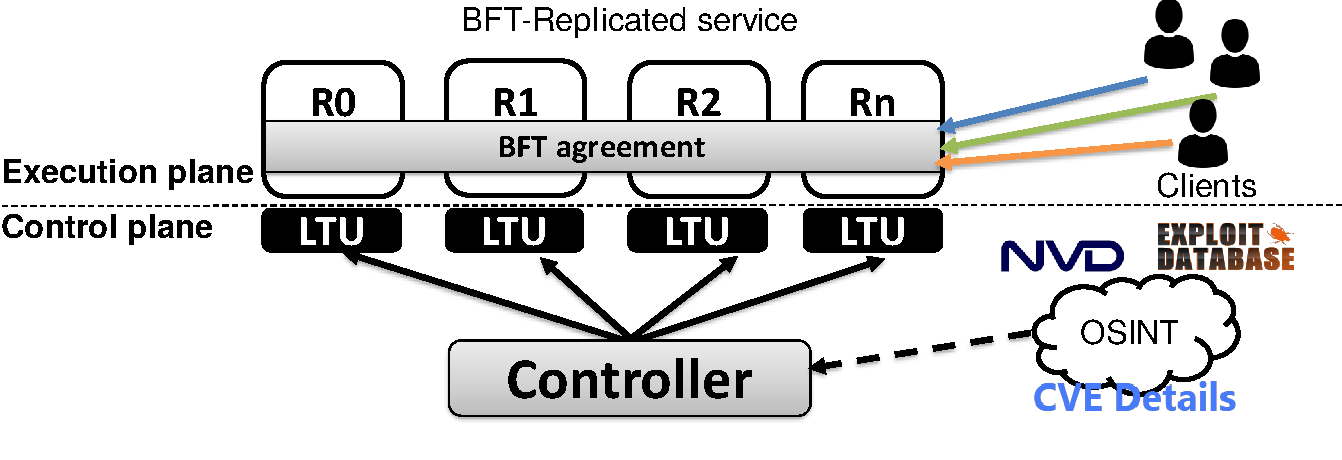
\includegraphics[width=0.7\columnwidth]{images/images/overview.pdf}
\vspace{-5mm}
\caption{\system overview.}
\label{fig:overview}
\end{center}
\end{figure}


\section{System Model}
\label{sec:systemmodel}

\system system model shares some similarity with previous works on the proactive recovery of \gls{bft} systems (e.g.,~\cite{Castro:2002,Platania:2014,Sousa:2010,Roeder:2010}).
More specifically, we consider a \emph{hybrid system model} composed of two planes with different properties and assumptions:

\begin{itemize}

\item \textbf{Execution Plane:} 
This plane is componsed of replica processes that can be subject to Byzantine failures.
Therefore, a Byzantine replica can try to mislead the other replicas or the clients.
These replicas communicate through an asynchronous network that can delay, drop or modify messages, just like most \gls{bft} system models~\cite{Castro:1999,Kotla:2010,Bessani:2014,Aublin:2015}.
This plane hosts $n$ replicas from which at most $f$ can be compromised at any given moment.
In this paper, we consider the typical scenario in which $n=3f+1$~\cite{Castro:2002,Kotla:2010,Aublin:2015}.  

\item \textbf{Control Plane:}  
For simplicity, we will address this component as a logical-centralized controller, which requires stronger assumptions. 
However, in Chapter~\ref{} we introduce \controller which requires weaker assumptions like the Execution Plane.

In this plane, we assume that each component can only fail by crashing. 
Each \emph{node} hosting processes contains a \gls{ltu}, and there is a logically-centralized controller to reconfigure the system, just like what has been used in several previous works on proactive recovery (e.g.,~\cite{Roeder:2010,Platania:2014,Sousa:2010}).
The failures of such components do not compromise the liveness and safety of the service as long as the control plane is recovered before $f$ replicas fail.


\end{itemize}

Besides the execution and control planes, we assume the existence of two types of external components: (1) clients of the replicated service, which can be subject to Byzantine failures; (2) \gls{osint} sources (e.g., \gls{nvd}, ExploitDB) that can not be subverted and controlled by the adversary.
In practice, this assumption lead us consider only well-established and authenticated data sources.
Dealing with untrusted sources is an active area of research in the threat intelligence community (e.g.,~\cite{Sabottke:2015,Liu:2015}), which we consider out of scope for this paper.


\section{Execution Plane}
\label{sec:executionplane}

The Execution Plane can accomodate any replicated system that already levareges on the existence of a controller node (e.g.,~\cite{Sousa:2010,Roeder:2010,Platania:2014,Garcia:2016}) or any \gls{bft} system that would benefit from the \system assistence (e.g.,~\cite{Sousa:2018}). 
However, a few requriements must be fulfilled, the Execution Plane is supported by virtulization therefore the \gls{bft} must run in a \gls{vm}.
Additionally, the \gls{bft} library must provide replicas configuration in order to allow replicas' replacement.
In this thesis we evaluate \system with three instances of differente Execution Planes: \gls{bft} ordering for Hyperledger Fabric, a \gls{kvs}, and \sieveq.
The latter, is one of the contributions of the thesis (see Chapter~\ref{chap:sieveq} and Chapter~\ref{chap:sieveqevaluation}, therefore detail its description.


\sieveq provides a message queue abstraction for critical services, applying various filtering rules to determine if messages are allowed to go through.
\sieveq is not a conventional firewall and we do not claim that it should replace existing firewalls in all deployment scenarios.
We are focusing on service- or information-critical systems that require a high-level of protection, and therefore, justify the implementation of advanced replication mechanisms.
The system we propose is able to deliver messages while guaranteeing authenticity, integrity, and availability.
As a consequence, and in contrast to conventional firewalls, we lose transparency on senders and receivers, since they are aware of the \sieveq's end-points.
The rest of the section explains how we address some of the mentioned issues and introduces the main design choices and the architecture of \sieveq.




Typical resilient firewall designs are based on primary-backup replication, and consequently, they are able to tolerate only crash failures.
Therefore, more elaborated failure modes may allow an adversary to penetrate into the protected network.


Some organizations deal with crashes (or \gls{dos} attacks) by resorting to several firewalls to support multiple entry points. 
This solution is helpful to address some (accidental) failures, but is incapable of dealing with an intrusion in a firewall.
In this case, the adversary gains access to the internal network, enabling an escalation of the attack, which at that stage can only be stopped if other protection mechanisms are in place.


Different fault tolerance mechanisms are employed at the two stages. 
Pre-filtering is implemented by a dynamic group of nodes named \presieves. 
\Presieves can be the target of various kinds of attacks and eventually may be intruded because they face the external network. Therefore, we take the conservative approach of assuming that \presieves can fail in an arbitrary (or Byzantine) way, meaning that they may crash or start to act maliciously.
When a failed \presieve is detected, it is simply replaced by a new one that is clean from errors.
Since \sieveq needs to support different message loads, e.g., due to additional senders, \presieves can be created dynamically to amplify the aggregated processing capabilities (within the constraints of the hardware).
The filtering stage is performed by a group of \repsieve components, which execute as a replicated state machine~\cite{Schneider:1990}.
\Repsieves may also fail in an arbitrary way, and therefore, we employ an intrusion-tolerant replication protocol that ensures correct operation in the presence of Byzantine faults.

Our solution was guided by the following design principles:

\begin{itemize}

\item \emph{Application-level filtering}: support sophisticated firewall filtering rules that take advantage of application knowledge. \sieveq implements this sort of rules by maintaining state about the existing flows, and this state has to be consistently replicated using a \gls{bft} protocol.

\item \emph{Performance}: address the most probable attack scenarios with highly efficient approaches, and as early as possible in the filtering stages; Reduce communication costs with external senders, as these messages may have to travel over high latency links (e.g., do not require message multicasts).	

\item \emph{Resilience}: tolerate a broad range of failure scenarios, including malicious external/internal attackers, compromised authenticated senders, and intrusions in a subset of the \sieveq components; Prevent malicious external traffic from reaching the internal network by requiring explicit message authentication.

\end{itemize}



\section{Control Plane}
\label{sec:controlplane}

\system is the first control plane that automatically changes the attack surface of a \gls{bft} system in a dependable way.
\system continuously collects security data from \gls{osint} feeds on the internet to build a knowledge base about the possible vulnerabilities, exploits, and patches related to the systems of interest.
This data is used to create clusters of similar vulnerabilities, which potentially can be affected by (variations of) the same exploit.
These clusters and other collected attributes are used to analyze the risk of the \gls{bft} system becoming compromised. % due to common vulnerabilities.
Once the risk increases, \system replaces the potentially vulnerable replica by another one, trying to maximize the failure independence. % of the replicated service.
Then, the replaced node is put on quarantine and updated with the available patches, to be re-used later.
These mechanisms were implemented to be fully automated, removing the human from the loop.

The current implementation of \system manages 17 \gls{os} versions, supporting the \gls{bft} replication of a set of representative applications.
The replicas run in \glspl{vm}, allowing provisioning mechanisms to configure them. 
We conducted two sets of experiments, one demonstrates that \system risk management can prevent a group of replicas from sharing vulnerabilities over time; the other, reveals the potential negative impact that virtualization and diversity can have on performance. 
However, we also show that if naive configurations are avoided, \gls{bft} applications in diverse configurations can actually perform close to our homogeneous bare metal setup.

\subsection{BFT-Control Plane}
\note{add details later}

\section{Diversity of Replicas}
\label{sec:diversityofreplicas}
\note{citar survey \cite{Baudry:2015}}
%BFT-replicated services running on \system are composed by $n$ replicas.
For our purposes, each \replica is composed of a stack of software, including an OS (kernel plus other software contained in an \gls{os} distribution), execution support (e.g., \gls{jvm}, \gls{dbms}), a \gls{bft} library, and the service that is provided by the system.
%(see Figure~\ref{fig:arch1}).
The set of $n$ replicas is called a \configuration.

It is possible to improve the \replicas fault independence by resorting to different \gls{ots} components in the software stack~\cite{Deswarte:1998}. 
For example, it has been shown that using distinct \glspl{os}~\cite{Garcia:2014}, filesystems~\cite{Rodrigues:2001,Bairavasundaram:2009}, and databases~\cite{Gashi:2007}, can yield important benefits in terms of fault independence. In addition, automatic techniques could enhance diversity, like randomization/obfuscation of \glspl{os}~\cite{Roeder:2010} and applications~\cite{King:2016}.

Although \system can exploit automatic techniques, in this paper we center our attention on diverse \gls{ots} components. 
In particular, \system monitors the disclosed vulnerabilities of all elements of the software stacks of the replicas to assess which of them may contain common vulnerabilities.  

However, in the experimental evaluation, we focus on the diversity of OSes (not only the kernel, but the whole product) for three fundamental reasons: (1) by far, most of the replica’s code is the \gls{os}; (2) such size and importance, make \glspl{os} a valuable target, with new vulnerabilities and exploits being discovered every day; and (3) there are many options of OSes that can be used.
The two last factors are particularly important to enrich the validity of our analysis.

Moreover, we do not explicitly consider the diversity of the \gls{bft} library (i.e., the protocol implementation) or the service code implemented on top of it.
Four facts justify this decision: (1) N-version programming is too costly for this~\cite{Avizienis:1977}; (2) there have been some works showing that such protocol implementations can be generated from formally verified specifications~\cite{Hawblitzel:2015,Rahli:2018}; (3) the relatively small size of such components (e.g., a key-value store on top of BFT-SMaRt has less than 15k lines of code~\cite{Bessani:2014}) make them relatively simple to test and assess with some confidence~\cite{Martins:2013,Lee:2014};  and (4) there are no reported vulnerabilities about these system to support our study.
Notice that, although we do not explicitly consider the diversity of \gls{bft} libraries, nothing prevents \system from monitoring them (when several alternatives become available). 
Additionally, as a pragmatic approach, we could employ automatic diversity techniques in this layer~\cite{Platania:2014,Roeder:2010}.



\chapter{\sieveq}
\label{chap:sieveq}

\chapter{Finding evidence for supporting and manage diversity }
\label{chap:supportingdiversitymechanism}

 \note{We need to clarify that \system is proactive and \sieveq is reactive, they can be used together. E.g., when there is a problem the controller increases the risk}
\section{Introduction}

Practical \gls{bft} replication was initially proposed as a solution to handle Byzantine faults of both accidental and malicious nature~\cite{Castro:1999}.
The correctness of a BFT service comes from the existence of a quorum of correct nodes, capable of reaching consensus on the (total) order of messages to be delivered to the replicas.
For instance, to tolerate a single replica failure, the system typically must have four replicas~\cite{Castro:2002,Kotla:2010,Aublin:2015}. 
This model only works if nodes fail independently, otherwise, once an attacker discovers a vulnerability in one node, it is most likely that the remaining nodes suffer from the same weakness. 

In the last twenty years of \gls{bft} replication research, few efforts were made to justify or support this assumption. 
However, there were great advances on the performance (e.g.,~\cite{Kotla:2010,Aublin:2015,Behl:2015}), use of resources (e.g.,~\cite{Veronese:2013,Behl:2017,Liu:2016,Yin:2003}), and robustness (e.g.,~\cite{Amir:2011,Bessani:2014,Clement:2009b}) of BFT systems.
These works assume, either implicitly or explicitly, that replicas fail independently, relying on some orthogonal mechanism (e.g.,~\cite{Roeder:2010,Chen:1995}) to remove common weaknesses, or rule out the possibility of malicious failures from their system models.
A few works have implemented and experimented such mechanisms~\cite{Rodrigues:2001,Roeder:2010,Amir:2011}, but in a very limited way.
Nonetheless, in practice, diversity is a fundamental building block of dependable services in avionics~\cite{Yeh:2004}, military systems~\cite{rhimes}, and even in recent blockchain platforms such as Ethereum\footnote{\url{https://www.reddit.com/r/ethereum/comments/55s085/geth_nodes_under_attack_again_we_are_actively/}} -- three essential applications of \gls{bft}. 

For the few works that do consider the diversity of replicas, the absence of common-mode failures is mostly taken for granted.
For example, by using memory randomization techniques~\cite{Roeder:2010} or different OSes~\cite{Rodrigues:2001,Junqueira:2005}, it is assumed that such failures will not exist without providing evidence for it. 
In fact, researchers have argued that randomization techniques do not suffice to create fault independence~\cite{Snow:2013,Bittau:2014}.
In addition, although the use of distinct OSes promotes fault independence to some extent, \emph{per se} it is not enough to preclude vulnerability sharing among diverse \glspl{os}~\cite{Garcia:2014}.

Even if there was an initial diverse set of $n$ replicas that would have fault independence, long-running services eventually will need to be cleaned from possible failures and intrusions.
Proactive recovery of \gls{bft} systems~\cite{Castro:2002,Sousa:2010,Roeder:2010,Platania:2014,Distler:2011} periodically restarts the replicas to remove undetected faulty states introduced by a stealth attacker. 
However, a common limitation is that these works assume that the weaknesses will be eliminated after the recovery.
In practice, this does not happen unless the replica code changes after its recovery.

This paper presents \system, 
%a control plane integrated with BFT replication.
%It is the first to apply techniques from MTD to automatically change the attack surface of BFT systems in a dependable and automatic way.
%It is 
the first system that automatically changes the attack surface of a \gls{bft} system in a dependable way.
\system continuously collects security data from \gls{osint} feeds on the internet to build a knowledge base about the possible vulnerabilities, exploits, and patches related to the systems of interest.
This data is used to create clusters of similar vulnerabilities, which potentially can be affected by (variations of) the same exploit.
These clusters and other collected attributes are used to analyze the risk of the \gls{bft} system becoming compromised. % due to common vulnerabilities.
Once the risk increases, \system replaces the potentially vulnerable replica by another one, trying to maximize the failure independence. % of the replicated service.
Then, the replaced node is put on quarantine and updated with the available patches, to be re-used later.
These mechanisms were implemented to be fully automated, removing the human from the loop.

The current implementation of \system manages 17 \gls{os} versions, supporting the \gls{bft} replication of a set of representative applications.
The replicas run in \glspl{vm}, allowing provisioning mechanisms to configure them. 
We conducted two sets of experiments, one demonstrates that \system risk management can prevent a group of replicas from sharing vulnerabilities over time; the other, reveals the potential negative impact that virtualization and diversity can have on performance. However, we also show that if naive configurations are avoided, \gls{bft} applications in diverse configurations can actually perform close to our homogeneous bare metal setup.
%These results open avenues for many future works in the area. 

In summary, we make the following contributions: 

\begin{enumerate}

\item \system, a control plane that monitors \gls{osint} data and manages the \gls{bft} service replicas, selecting and reconfiguring the system to always run the ``most diverse'' set of replicas at any given time (Sections~\ref{sec:design} and~\ref{sec:implementation});

\item A method for assessing the risk of a group of replicas being compromised based on the security news feeds available on the internet. 
The method overcomes limitations from works that use NVD data for managing the replicas vulnerability independence (Section~\ref{sec:metric});

\item An evaluation of our risk management method based on real historical vulnerability data showing its effectiveness in keeping a group of replicas safe from common vulnerabilities (Section~\ref{sec:diversity});

\item An extensive evaluation of \system prototype using 17 \gls{os} versions, a \gls{bft} replication library, and some \gls{bft} applications (i.e., a \gls{kvs}, an application-level firewall/message queuing service, and a blockchain service) showing the costs of supporting diversity in \gls{bft} systems (Section~\ref{sec:overhead}).

\end{enumerate}


\section{Diversity-aware Reconfigurations}
\label{sec:metric}

The core of \system is the vulnerability evaluation method used to assess the risk of having replicas with shared vulnerabilities.
This section details this method.

\subsection{Finding Common Vulnerabilities}

\gls{nist}'s \gls{nvd}~\cite{nvd} is the authoritative data source for disclosure of vulnerabilities and associated information~\cite{Massacci:2010}. 
\gls{nvd} aggregates vulnerability reports from more than 70 security companies, advisory groups, and organizations, thus being the most extensive vulnerability database on the web. 
All data is made available as \gls{xml} data feeds, containing the reported vulnerabilities on a given period. 
Each \gls{nvd} vulnerability receives a unique identifier and a short description provided by the \gls{cve}~\cite{cveterm}. 
The \gls{cpe}~\cite{cpe} provides the list of products affected by the vulnerability and the date of the vulnerability publication.
The \gls{cvss}~\cite{cvss} calculates the vulnerability severity considering several attributes, such as the attack vector, privileges required, exploitability score, and the security properties compromised by the vulnerability (i.e., integrity, confidentiality, or availability).

Previous studies on diversity solely count the number of shared vulnerabilities among different \glspl{os}, assuming that less common vulnerabilities implies a smaller probability of compromising $f+1$ OSes~\cite{Garcia:2014}. 
Although this intuition may seem acceptable, in practice it underestimates the number of shared vulnerabilities due to imprecisions in the data sources. 
For example, Table~\ref{tab:missing_products} shows three vulnerabilities, affecting three different \glspl{os} at distinct dates.
At first glance, one may consider that these \glspl{os} do not share vulnerabilities.
However, a careful inspection of the descriptions shows that they are very similar.
Moreover, we checked this resemblance by searching for additional information on security web sites, and we found out that CVE-2016-4428, for example, also affects Solaris.\footnote{\url{https://www.oracle.com/technetwork/topics/security/bulletinjul2016-3090568.html}}

\begin{table}[!t]
\begin{center}
{\scriptsize
\begin{tabular}{| p{2.3cm} | p{10cm} | }\hline
\textbf{CVE (affected OS)} & \textbf{Description} \\\hline\hline
CVE-2014-0157 (Opensuse 13) & \scriptsize \gls{xss} vulnerability in the Horizon Orchestration dashboard in OpenStack Dashboard (aka Horizon) 2013.2 before 2013.2.4 and icehouse before icehouse-rc2 allows remote attackers to inject arbitrary web script or HTML via the description field of a Heat template. \\ \hline
CVE-2015-3988 (Solaris 11.2) & \scriptsize Multiple \gls{xss} vulnerabilities in OpenStack Dashboard (Horizon) 2015.1.0 allow remote authenticated users to inject arbitrary web script or HTML via the metadata to a (1) Glance image, (2) Nova flavor or (3) Host Aggregate. \\ \hline
CVE-2016-4428 (Debian 8.0) & \scriptsize \gls{xss} vulnerability in OpenStack Dashboard (Horizon) 8.0.1 and earlier and 9.0.0 through 9.0.1 allows remote authenticated users to inject arbitrary web script or HTML by injecting an AngularJS template in a dashboard form. \\ \hline
\end{tabular}
}
\caption{Similar vulnerabilities affecting different OSes.}
\label{tab:missing_products}
\end{center}
\end{table}

Even with these imperfections, \gls{nvd} is still the best data source for vulnerabilities.
Therefore, we exploit its curated data feeds for obtaining the unstructured information present in the vulnerability text descriptions and use this information to find similar weaknesses.
A usual way to find similarity in unstructured data is to use clustering algorithms~\cite{Jain:2010}.
Clustering is the process of aggregating related elements into groups, named clusters, and is one of the most popular unsupervised machine learning techniques. 
We apply this technique to build clusters of similar vulnerabilities (see Section~\ref{sec:details} for details), even if the data feed reports that they affect different products.
For example, the vulnerabilities in Table~\ref{tab:missing_products} will be placed in the same cluster as there is some resemblance among the descriptions, and they can potentially be activated by (variations of) the same exploit.

It is worth to remark that by using clusters to find similar vulnerabilities, we conservatively increase the chances of capturing shared weaknesses contributing to the score of a pair of replicas.

\subsection{Measuring risk}
\label{sec:measurerisk}

As discussed before, each vulnerability in \gls{nvd} has an associated \gls{cvss} severity score. 
Therefore, a straw man solution for measuring risk would be to sum the \gls{cvss} scores of all common vulnerabilities in the software stack of two replicas to get an estimate of how dangerous are their shared weaknesses.
However, \gls{cvss} has some limitations that make it unsuitable for managing the risk of replicated systems:
(1) In practice, it has been shown that there is no correlation between the \gls{cvss} exploitability score and the existence of real exploits for the vulnerability~\cite{Bozorgi:2010}; 
(2) \gls{cvss} does not provide information about vulnerabilities exploiting and patching times; 
(3) \gls{cvss} does not account for the vulnerability age, which means that severity remains the same over the years~\cite{Frei:2006}; 
and (4) some studies show that \gls{cvss} may overestimate  severity~\cite{Sabottke:2015}, as for example larger scores do not correspond to higher prices in the vulnerabilities' black markets~\cite{Allodi:2014}.

Given these limitations, we derive a novel, more refined, metric to measure the risk of a \gls{bft} system being affected by common vulnerabilities.
In our particular context, we are mostly interested in capturing information that relates to the window of exposure that vulnerabilities have, mainly when they are correlated among \replicas.
Therefore, we developed a risk metric that aims to overpass the identified limitations. 
We solved (1) and (2) by using additional \gls{osint} sources that provide information about the exploit and patch dates. 
Since NVD does not provide this information, we collect more data from other \gls{osint} sources like Exploit-DB~\cite{edb} for exploits, patching information from CVE-details~\cite{cvedetails}, and additional vendor websites, such as Ubuntu Security Notices~\cite{ubuntu}, Debian Security Tracker~\cite{debian}, and Microsoft Security Advisories and Bulletins~\cite{microsoft} (which also give additional product versions affected by the vulnerability).
We solve (3) using the vulnerability published date to calculate its age.
Finally, we only use the \gls{cvss} attributes that concern to integrity and availability, the properties traditionally related with \gls{bft} replication (4).



\begin{table}[h]
\begin{center}
{\small
\begin{tabular}{ c }\hline
\vbox{
\begin{equation}
\mathit{\systemformula(sc)}=\sum_{i=1}^{n-1} \sum_{j=i+1}^{n} \pairformula(rc_i,rc_j) \label{eq:3}
\end{equation}
}\\ \hline
\vbox{
\begin{equation}
\mathit{\pairformula(rc_i,rc_j)}=\sum_{v_k \in \mathcal{V}_{i,j}} \mathit{\vulnerabilityformula(v_k)} \label{eq:2}
\end{equation}
}\\ \hline
\vbox{
\begin{equation}
\mathit{\vulnerabilityformula(v_k)}= (A+I+\mathit{exp(v_k)}) \times \mathit{tdist(v_k)} \label{eq:1}
\end{equation}
\begin{equation}

\mathit{exp(v_k)}= \begin{cases}
		\mathit{max(\mathit{DP}-\mathit{DE},0)}+1 	& \text{$v_k$ exploited, patched}\\
  		\mathit{DE} 		& \text{$v_k$ exploited, not patched}\\
		0 		& \text{otherwise}
\end{cases} \label{eq:exposed}
\end{equation}
}\\ \hline

\end{tabular}
}
\label{tab:equations}
\end{center}
\end{table}

Our metric considers all this information to measure the risk of a set of $n$ replicas having active shared vulnerabilities.
More specifically, it works as an indicator of how fault-independent is a \configuration.
Equation~\ref{eq:3} shows the risk of a \configuration as the sum of the different \replica pairs' score.
This score is calculated based on the set of vulnerabilities $\mathcal{V}_{i,j}$ that affects both $r_i$ and $r_j$ or that are present in a cluster containing vulnerabilities affecting both \replicas (Equation~\ref{eq:2}).
Finally, we calculate the score of each vulnerability in $\mathcal{V}_{i,j}$ (Equation~\ref{eq:1}). 
We assign a \emph{dynamic score} to each vulnerability, considering the referred attributes:
\emph{(i)} we take two \gls{cvss} attributes to capture the extent to which a vulnerability $v_k$ affects availability ($A$) and integrity ($I$);
\emph{(ii)} we account for the number of days the vulnerability was exposed with $\mathit{exp}$, i.e., there was an exploit and no patch available.
This is calculated considering the number of days to patch ($DP$) and to exploit ($DE$) $v_k$ (Equation~\ref{eq:exposed}); 
\emph{(iii)} and we use an amortization function to reflect the fact that older vulnerabilities have are less likely to harm the system ($\mathit{tdist(v_k)} \in [0,1]$).


\subsection{Selecting Configurations}
\label{sec:configurations}


We use the risk metric to choose the \replicas that should be included in the \configuration. 
This is done by periodically evaluating the risk of the current \configuration. 
If the risk exceeds a pre-defined threshold, a mechanism is triggered to replace replicas and reduce the overall risk.
First, it decides which \replica (\r) should be removed and put in a quarantine set (\QS). 
Then, it selects (one of) the best candidate(s) replicas from all the available candidates (\RS) to make the substitution.
When the replacement takes place, the resulting \configuration (\ES) has lower risk than the previous one.
Additionally, we ensure that removed \replicas can sometime later re-enter the system, and the ones that are in the system, despite their overall score, are eventually replaced.
Therefore, each replica \r in \ES has an \emph{age} value that is incremented. 
On the contrary, each removed replica \r in \QS, has a \emph{healing} value that is decremented.


This procedure is detailed in Algorithm \ref{alg:algorithm2}.
The \emph{Monitor} function is called on each monitoring round (e.g., on every hour).
Consider a \ES that is already running with risk$=\alpha$.
First, the algorithm increments the \emph{age} of each \r in \ES (lines 6-7).
Then, it verifies if the risk of \ES (Equation~\ref{eq:3}) does not exceed the predefined $\mathit{threshold}$ (line 8).
In the affirmative case, a \replica replacement is started.
First, some local variables are initialized (lines 9-10).
Second, it randomly gets pairs $\langle i,j \rangle$ from \ES (line 11) and saves some of them that augment the risk in \MAX (Equation~\ref{eq:2}) (lines 12-14). 
Third, the algorithm picks the older replica (i.e., the one that is in \ES for more time) of all selected pairs (lines 15-18). 
This replica is removed from \ES (line 19) and added to \QS (line 21).
The \emph{healing} value is initialized with a value, different for each \replica, based on historical data about the time it takes for a patch to be published for this software (line 20). 
The algorithm calls a function that selects a new replica to join \ES (line 22). Finally, it decrements the \emph{healing} of each \r in \QS (line 24). When such value reaches zero, \r is removed from \QS and added to \RS (lines 25-28).

Function \emph{Find\_new\_config()} (line 22) solves the following optimization problem:

\vbox{
\begin{small}
\begin{equation*}
\begin{array}{ll@{}ll}
\text{\underline{min} } & \emph{risk}(\ES \cup \{r\}) 	 	\\
\text{\underline{subject to}}	&	 r \in \RS 			\\ 
\end{array}
\end{equation*}
\end{small}
}

\noindent
where \ES is the set of $n-1$ replicas that will stay in the system and $r$ is the new replica (which we have to find) among the ones in \RS.
The twist in our case is that we avoid deterministic solutions to increase the difficulty of an adversary guessing the next configurations.
Therefore, we developed a simple heuristic that finds the $k$ best replicas in \RS (e.g., $k=3$) and randomly picks one of them to be added to \ES.
The heuristic is quite simple: we just calculate the risk of a configuration with each candidate replica from \RS, and choose one of the $k$ replicas that induce lower risk. 

%The minimization problem presented is similar to a problem of solving the minimal cost of a $n$-clique for complete graphs. 
%However, as we mentioned before, we want to create unpredictability on the results.
%Therefore, we introduce randomness on the selection, meaning that the solution is minimal but not always the minimum.
%The minimization function (line 22) is a heuristic to select the valid candidates to reconfigure the \ES with a smaller $\alpha$ than before. 
%The selection of \r must have some degree of unpredictability to increase the difficulty of guessing future configurations.
%To meet this goal, we add randomness when picking \replicas while restricting the number of candidate elements to the ones that minimize the risk. 
%It starts iterating over the \RS and uses the Equation~\ref{eq:3} to calculate the risk of such configuration (line 30).
%If the risk is under a predefined $threshold$, the candidate \r is initialized (line 32), removed from the \RS (line 33) and added to a set with the admissible candidates (\PS) (line 34).
%Then, a random \r is picked from \PS and added to \ES (line 35) which is then returned (line 36).

Although better heuristics can be developed, this brute-force method works in \system because we do not expect \RS (our solution space) to be large.
In addition, this function is only called  if the risk exceeds the threshold. 

\begin{algorithm}[t]
\caption{Replica Set Reconfiguration}\label{alg:algorithm2}
{\footnotesize
%\N: number of replicas\;
%\K: number of replicas to remove\;
\ES: set replicas in the \configuration \;
\RS: set with the available replicas (not in use)\;
%\CS: set of candidate replicas\;
%\RM: set of removable replicas\;
\MAX: set of candidate replicas to remove\;
\QS: set of quarantine replicas\;
%\PS: set of valid replicas\;

\BlankLine
\Fn{Monitor ()}{
	\ForEach{r in \ES}{
		\Inc{r.age};
	}
	\If{\Risk{\ES} $>$ threshold}{
		$maxScore$, $maxAge$ $\leftarrow$ 0\;
		\toRemove $\leftarrow$ $\perp$\;
%		\While{\Size{\toRemove} $<$ \K}{
			\ForEach{$\langle i,j \rangle$ in \ES}{
				\If{\Common{i,j} $\geq$ maxScore}{	
					\MAX $\leftarrow$ \MAX $\cup$ $\{\langle i,j \rangle\}$\;
					$maxScore$ $\leftarrow$ \Common{i,j}\;
				} 
			}
				\ForEach{$\langle i,j \rangle$ in \MAX}{
					\If{\Older{i,j} $\geq$ maxAge}{	
						\toRemove $\leftarrow$ \Older{i,j}\;
						$maxAge$ $\leftarrow$ \toRemove.age\;	
					} 
			}		
			 \ES $\leftarrow$ \ES $\setminus$ $\{$ \toRemove$\}$\;	
             $\toRemove$.healing $\leftarrow$ \healing{\toRemove}\;
			 \QS $\leftarrow$ \QS $\cup$ $\{$ \toRemove$\}$\;
%		}
		 \ES $\leftarrow$ $\mathit{Find\_new\_config(\RS, \ES)}$\;
	}
	\ForEach{r in \QS}{
		\Dec{r.healing}\;
		\If{r.healing $=$ 0}{		
			\QS $\leftarrow$ \QS $\setminus$ $\{r\}$\;		
			$r.age$ $\leftarrow$ 0\;
            \RS $\leftarrow$ \RS $\cup$ $\{r\}$\;
		}
	}
}
%\Fn{Minimize (\RS, \ES)}{
%%	\If{\Size{\ES} is $\emptyset$}{
%%		\CS $\leftarrow$ $\emptyset$\;
%%		\CS $\leftarrow$ \Rand{\RS}\; 
%%	}
%%	\While{\Size{\CS} $\leq \N$}{
%		\PS $\leftarrow$ $\{\}$\;
%		\ForEach{r in \RS}{
%			\If{\Risk{\ES $\cup$ r} $<$ threshold}{
%				r.age $ \leftarrow$ 0\;
%				\RS $\leftarrow$ \RS $\setminus$ $\{r\}$\;		
%				\PS $ \leftarrow$ \PS $\cup$ $\{r\}$\;
%			}
%		}
%		\ES $\leftarrow$ \ES $\cup$ $\{\Rand{\PS}\}$\;
%%	}
%\Return	\ES\;
%}
%\end{multicols}
}
\end{algorithm}


\section{\system Implementation}
\label{sec:implementation}

This section details the implementation of each component of \system. 
It also briefly presents other aspects of our prototype.% like the management of replicas running in a virtualized environment.


\subsection{Control Plane}
\label{sec:lazarus}

Figure~\ref{fig:arch1} shows \system control plane with its four main modules, described below.

\begin{figure}[h]
\begin{center}
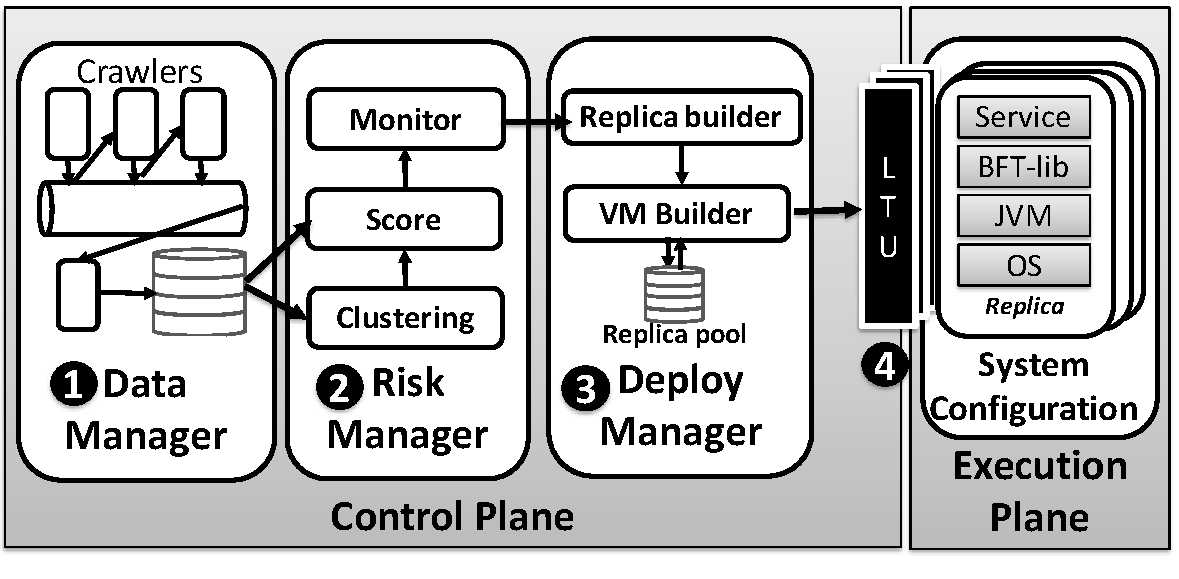
\includegraphics[width=.9\columnwidth]{images/images/architecture_new.pdf}
\vspace{-5mm}
\caption{\system architecture.}
\vspace{-5mm}
\label{fig:arch1}
\end{center}
\end{figure}


\circled{1} \textbf{\fetcher.} \system needs to know the software stack of each available replica to be able to look for vulnerabilities in this software.
The list of software products is provided following the \gls{cpe} Dictionary~\cite{cpe}, which is also used by \gls{nvd}. 
%The \fetcher determines if the CPE list is updated by checking the most recent CPE count in the NVD web page.
For each software, the administrator can indicate the time interval (in years) during which data should be obtained from \gls{nvd}' feeds.

The \fetcher parses the \gls{nvd} feeds considering only the vulnerabilities that affect the chosen products. 
The processing is carried out with several threads cooperatively assemblying as much data as possible about each vulnerability -- a queue is populated with requests pertaining a particular vulnerability, and other threads will look for related data in additional \gls{osint} sources. 
Typically, the other sources are not as well structured as \gls{nvd}, and therefore they have to be handled with specialized HTML parsers that we have developed. 
Currently, the prototype supports five other sources, namely Exploit DB, CVE-details, Ubuntu, Debian, and Microsoft. 
As previously mentioned, such sources provide complementary data, like additional affected products versions not mentioned in \gls{nvd}.

The collected data is stored in a relational database (MySQL).
For each vulnerability we keep its \gls{cve} identifier, the published date, the products it affects, its text description, some \gls{cvss} attributes (e.g., availability and integrity); and exploit and patching dates.


\circled{2} \textbf{\risk.} This component finds out when it is necessary to replace the currently running group of \replicas and discovers an alternative configuration that decreases the risk. 
As explained in Section~\ref{sec:measurerisk}, the risk is computed using score values that require two kinds of data: the information about the vulnerabilities, which is collected by the \fetcher; and the vulnerability clusters. 
A vulnerability cluster is a set of vulnerabilities that are related accordingly to their description (see Section~\ref{sec:details} for details).
The \risk also runs Algorithm~\ref{alg:algorithm2} to monitor the replicated system and trigger reconfigurations.


\circled{3} \textbf{\manager.} 
This component automates the setup and execution of the diverse replicas. 
It creates and deploys the \replicas in the execution environment implementing the decisions of the \risk, i.e., it dictates when and which \replicas leave and join the system. 
We developed a replica builder on top of Vagrant~\cite{vagrant}.
It is responsible for downloading, installing, and configuring the \replicas.
Moreover, it performs replica maintenance, where  \replicas in \QS are booted to carry out automatic software updates (i.e., patching). 


\paragraph{Setup.}
The box configuration is defined in a configuration file, named \emph{Vagrantfile}, consider the example in Listing~\ref{vagrantfile}.
In this file, it is possible to set several options of the box, to name a few:
the box name, the number of CPUs, the amount of memory RAM, the IP, the type of network, sync folders between host and the box, etc. 
Additionally, it is possible to pass some VM-specific parameters, e.g., some CPU/mother board flags such as enabling VT-x technology -- consider the \texttt{modifyvm} fields in Listing~\ref{vagrantfile} (lines 6-14).
It is possible to select different \gls{vm} providers (e.g., libvirt, VMware, VirtualBox, Parallels, Docker, etc), we rely on VirtualBox since it is the one with more diversity opportunities in the Vagrant Cloud~\cite{vagrantcloud}. 
Vagrant Cloud is a website that offers a plethora of different VMs.

\begin{lstlisting}[style=mystyle,caption=Windows Server 2016 Vagrantfile,label=vagrantfile]
Vagrant.configure(2) do |config|
	config.vm.box = "geerlingguy/ubuntu1604"
	config.ssh.insert_key = false
	config.vm.provider "virtualbox" do |v|
		v.customize ["modifyvm", :id, "--cpus", 4]
		v.customize ["modifyvm", :id, "--memory", 22000]
		v.customize ["modifyvm", :id, "--cpuexecutioncap", 100]
		v.customize ["modifyvm", :id, "--ioapic", "on"]
		v.customize ["modifyvm", :id, "--hwvirtex", "on"]
		v.customize ["modifyvm", :id, "--nestedpaging", "on"]
		v.customize ["modifyvm", :id, "--pae", "on"]
		v.customize ["modifyvm", :id, "--natdnshostresolver1", "on"]
		v.customize ["modifyvm", :id, "--natdnsproxy1", "on"]
	end
	config.vm.network "public_network", ip:"192.168.2.50", bridge:"em1"
	config.vm.provision :shell, path: "run_debian.sh", privileged: true
end
\end{lstlisting}

\todo{Add all fields that are mentioned, then add lines to the text}

\paragraph{Download.}
One of the fields of the \emph{Vagranfile} is the boxname, the \texttt{box} field is the key that is used to choose which box will be downloaded, each key is unique for each box.
There are plenty of \glspl{os} and versions ready-to-use, and the same OS/version can have different ``manufacturers" -- some of which are official.

\paragraph{Deploy and provision.}
Vagrant supports complex provisions mechanisms, such as Chef or Puppet, but shell script was sufficient for us. 
This is set in the \emph{Vagranfile} \texttt{provision} field, one can describe the provision steps inline or in an external file and link it to the \emph{Vagranfile}.
Then, when the OS is booting, after the basic setup, the \glspl{os} will execute the provision script.
In this script, we program which software will be downloaded and run in the \glspl{vm} and what configurations are needed. 
We have developed shell scripts for each \glspl{os}, some of which share the same script as Debian and Ubuntu. 
Each \glspl{os}, especially the ones from different \glspl{os} families (e.g., Solaris and BSD) have different commands to execute the same instructions.
Although different, all scripts were meant to do the same thing:
First the script installs the software that is missing in the box -- this is not true for all OSes -- like Java 8, \texttt{wget}, \texttt{unzip}, and any additional software that one wants to install/run after the \glspl{os} boot.



\paragraph{Command and Control.}
There are some simple commands to boot and halt a box, e.g., \texttt{vagrant up} and \texttt{vagrant halt}. 
Vagrant also provides an ssh command (\texttt{vagrant ssh}) that allows the host to connect to the box. 
Our manager component makes the bridge between the \risk and the execution environment.
We developed an API on top of Vagrant, another level of abstraction made to manage replicated systems.


\circled{4} \textbf{LTUs.} Each node that hosts a replica has a Vagrant daemon (see details in next section) running on its trusted domain.
This component is isolated from the internet and communicates only with the \system controller through \gls{tls} channels.

\subsection{Additional Details}
\label{sec:details}

\textbf{Vulnerability Clustering.}
A few steps are carried out to create the vulnerability clusters. 
First, the vulnerability description needs to be transformed into a vector, where a numerical value is associated with the most relevant words (up to 200 words). 
This operation entails, for example, converting all words to a canonical form and calculating their frequency (less frequent words are given higher weights).
Then, the K-means algorithm is applied to build the clusters~\cite{Jain:2010}, where the number of clusters to be formed is determined by the elbow method~\cite{Thorndike:1953}. 
%Currently, it is set $K=200$.
%The algorithm assigns each vulnerability to the cluster with the minimum distance to the cluster center. 
%Then, it computes the cluster centroid, i.e., the average of each data attribute using only the members of a cluster. 
%Next, it calculates the distance of every vulnerability to the centroid, potentially placing them in close clusters. 
%The algorithm stops when there are no further exchanges between clusters.
%We used the elbow method~\cite{Thorndike53whobelongs} to determine the number of clusters to be formed, in our case was $200$ clusters.
We used the open-source machine learning library Weka~\cite{weka} to build the clusters. 


\subsection{Clustering}\label{sec:clustering}
Clustering is the process of aggregating elements into similar groups, named clusters. 
For example, two elements from the same cluster have a higher probability of being similar than two elements from different clusters. 
We apply this technique to build clusters of similar vulnerabilities.
One of the benefits of applying clustering techniques to vulnerability-data is that the algorithm does not need prior knowledge about the data.
It is the process alone that discovers the hidden knowledge in the data.
Each cluster is used as a hint that similar vulnerabilities are likely to be activated through the same or similar exploit.
We considered the vulnerability description and published date to find these similarities. 
In the end, it is expected that the clusters have a minimal number of elements that just represent the same or similar vulnerabilities.


In order to apply a clustering technique to our data, we need to follow some steps:

\paragraph{1) Data representation}
We transform the data that is stored in a database into a format that is readable by the clustering algorithm. 
Since we are using Weka~\cite{weka}, the data must be represented as \gls{arff}. 
Basically, this is a CSV file with some meta information, see Listing~\ref{list:arff}.

\begin{lstlisting}[style=mystyle,caption=ARFF file describing a vulnerability.,label=list:arff]
@RELATION vulnerabilities
@ATTRIBUTE cve string
@ATTRIBUTE description string
@ATTRIBUTE published_date date "yyyy-MM-dd"
@DATA
CVE-2017-3301, 'vulnerability in the solaris component of oracle sun systems products suite subcomponent kernel the supported version that is [...] attacks of this vulnerability can result in unauthorized update insert or delete access to some of solaris accessible data cvss v base score integrity impacts', '2017-01-27'
...more
\end{lstlisting}


This file contains all the vulnerabilities entries in the database. 
As we are interested in the vulnerability similarities, we select only the \gls{cve} identifier, the text, that contains the most relevant and nonstructured information, and the published date.
These attributes add meaning and temporal reference to the clustering algorithm.


\paragraph{2) Data preparation}
In general, machine learning algorithms do not handle raw data, then the data needs to be prepared:
First, we transform the \gls{cve} string into a number, basically, for each \gls{cve}, there is a real number that identifies each \gls{cve} unequivocally. 
This attribute is transformed in numeric values using \emph{StringToNominal} filter. 
Each \gls{cve} identifier is mapped to a numeric value.
Second, we transform the published date to a number format that Weka can handle using the \emph{NumericToNominal} filter.
Third, the text description must be transformed into a vector, the vector will represent the frequencies of each word in the whole document of strings. 
We used the \emph{StringToWordVector} to transform a text string into a vector of word weights, these weights represent the relevance of each word in the document.
This filter contains the following parameters:
\begin{itemize}
\item \textbf{TF- and IDF-Transform}, both set to true, TF-IDF stands for term frequency-inverse document frequency. 
This is a statistical measure used to evaluate how relevant a word is to a document in a collection. 
The relevance increases proportionally to the number of times a word appears in the document but is offset by the frequency of the word in the corpus. 
For example, words that appear in all vulnerability descriptions, are less relevant than the ones that appear more in few vulnerabilities.
\item \textbf{lowerCaseTokens}, convert all the words to lower case.
\item \textbf{minTermFreq}, set to -1, this will preserve any word despite their occurrences in the document.
\item \textbf{normalizeDocLength}, set to normalize all data.
\item \textbf{stopwords}, we define a stop word list, then words from this list are discarded. We begin with a general English stop word list containing pronouns, articles, etc. 
\item \textbf{tokenizer}, set to \emph{WordTokenizer}, this filter will remove special characters from the text, there is a default set of characters but we added a few more.
\item \textbf{wordsTopKeep}, is the number of words that will be kept to make the clusters. We kept $200$ as it was the number of words that represent better the lexical of vulnerabilities after removing the \emph{stopwords}.
\end{itemize}


Our goal is to build clusters in such way that similar vulnerabilities, even if they affect different products, are put together in the same cluster. 
For example, recall the vulnerabilities in Table~\ref{tab:missing_products}, which can be put in the same cluster since they are very similar.
Some of the parameters listed above needed some tuning to achieve our goals.
For example, before the tuning, some of the clusters were representing types of vulnerabilities, e.g., buffer overflow, cross-site scripting, etc. 
Since we are not interested in that type of clusters we have refined our \emph{stopword list} to reduce the description vocabulary to contain only what matters for us.
We have done this by iterating the process and checking the most used words (top 200 words) for clustering (this can be seen in Weka's intermediary output).
Then, we added the most relevant from the 200 words that were deviating from our goal.
In the end, we have a stop word list~\footnote{Stop word list is available: here} without the security-vocabulary noise.


When the pre-filtering ends, Weka presents a file very similar to the previous \gls{arff} file with the difference that the features are the most relevant words in the corpus. And each instance contains a value of relevance for each word.


\paragraph{3) Making clusters}
K-means is an unsupervised machine learning algorithm that groups data in K clusters.
The \emph{K-means} has two important parameters: the number of clusters to be formed, we set to $200$ clusters. We used the elbow method~\cite{Thorndike:1953} to decide $k=200$; and the \emph{distance function}, to calculate the distance between objects, the \emph{Euclidean Distance} is the most adequate for this type of data;
The \emph{K-means} computes the distance from each data entry to the cluster center (randomly selected in the first round).
Then, it assigns each data entry to a cluster based on the minimum distance (i.e., Euclidean distance) to each cluster center.
Then, it computes the centroid, that is the average of each data attribute using only the members of each cluster.
Calculate the distance from each data entry to the recent centroids. 
If there is no modification (i.e., re-arrangement of the elements in the cluster), then the clusters are complete, or it recalculates the distance that best fits the elements. 
When the K-means finishes the execution, we take the cluster assignments of each vulnerability. 
The assignments will be added to a new \gls{arff} file, similar to the first one but with a new attribute that is the cluster name (e.g., cluster1, cluster2, etc). 



Sometimes the resulting clusters include vulnerabilities that are unrelated. Therefore, we use the Jaccard index (J-index) to measure the similarity between the vulnerabilities within the cluster. We calculate the J-index of each element, and then the average J-index of the cluster. 
The clusters with a smaller average J-index (below a certain threshold) are considered ill-formed. In this case, we select the vulnerabilities with lower J-index and move them to another cluster that would result in a better J-index. If no such cluster exists, then we create a new one with the ``orphan'' vulnerability.

\textbf{BFT replication.}
Although there has been relevant research on \gls{bft} protocols over the last twenty years, there are few open-source replication libraries that implement them. \system can use any of those libraries, as long as they support replica set reconfigurations.
More specifically, to manage the \replicas, we need the ability to add first a new \replica to the set and then remove the old \replica to be quarantined. 
Therefore, we employ BFT-SMaRt~\cite{Bessani:2014}, a stable \gls{bft} library that provides reconfigurations on the \replicas set.

\textbf{Replica Virtualization.}
\glspl{vm} can be used to implement replicated systems, leveraging on the isolation between the untrusted and the trusted domains~\cite{Sousa:2010,Platania:2014,Distler:2011}.
Recovery triggering can be initiated from the isolated domain in a synchronous manner, reducing the downtime of the service during the reconfigurations. 
In our implementation, we resort to the Vagrant~\cite{vagrant} provisioning tool to do fast deployment of ready-to-use \glspl{os} and applications on \glspl{vm}. 
Vagrant supports several virtualization providers, e.g., VMware and Docker. 
From the available alternatives, we chose VirtualBox~\cite{virtualbox} because it offers more diversity opportunities, i.e., it supports a more extensive set of different guests \glspl{os}.
%The VMs are available in the Vagrant Cloud~\cite{vagrantcloud}.


\section{Evaluation of Replica Set Risk}
\label{sec:diversity}

This section evaluates how \system performs on the selection of dependable \replica configurations.
As discussed in Section~\ref{sec:replica}, we focus our experimental evaluation solely on the OS diversity.
% These play a crucial role in any IT system, and most of the \replica's code is the OS. 
% Thus, they present a high potential to become the most vulnerable part of a \replica.
% Hence, in the following experiments, we explore OS diversity among the replicas. 

In these experiments, we emulate live executions of the system by dividing the collected data into two periods:
(i) a \emph{learning phase} covering all vulnerability data between \emph{2010-1-1} and \emph{2017-9-29}, which is used to setup the \risk's algorithm; and (ii) an \emph{execution phase} composed of the period between \emph{2017-10-1} and \emph{2018-3-30}.
This last period is divided into three intervals of two months (OUT-NOV, DEC-JAN, and FEB-MAR), allowing for three independent tests.
%JAN-FEB, MAR-APR, and MAY-JUN
The goal is to create a knowledge base in the \emph{learning phase} that is used to assess \system choices during each interval of the \emph{execution phase}. 
A run starts on the first day of an interval and then progresses through each day of the interval until the end. Every day, we check if the currently executing replica set could be compromised by an attack exploring the vulnerabilities released on that day. 
We take the most pessimist approach, which is to say that we consider the system to be broken if a vulnerability comes out that affects at least two OSes that would be executing at that time.

Three additional strategies, inspired by previous works, were defined to be compared with \system (Section~\ref{sec:configurations}):

\begin{itemize}
\item \textbf{Equal:} all the replicas use the same randomly-selected OS during the whole execution. 
This strategy corresponds to the scenario where most past \gls{bft} systems have been implemented and evaluated (e.g.,~\cite{Kotla:2010,Aublin:2015,Behl:2015,Veronese:2013,Behl:2017,Liu:2016,Yin:2003,Amir:2011,Bessani:2014,Clement:2009b}). 
Here, compromising a replica would mean an opportunity to intrude the remaining ones.

\item \textbf{Static:} a configuration of $n$ different \glspl{os} is randomly selected, and there are no changes during the whole execution. 
This corresponds to a diverse \gls{bft} system without reconfigurations (e.g.,~\cite{Rodrigues:2001}).

\item \textbf{Random:} a configuration of $n$ \glspl{os} is randomly selected, and at the beginning of each day, a new \gls{os} is randomly picked to replace an existing one. 
This solution represents a system with proactive recovery and diversity, but with no informed strategy for choosing the next \configuration.

%\item \textbf{\system}, $n$ OSes are chosen based the algorithm described in Section~\ref{sec:measurerisk}. This algorithm decides when it is time to replace OSes, which OS is out and which OS is in.
\end{itemize}

The experiments consider a pool of 38 \gls{os} versions to be deployed on four replicas. 
At the beginning of the execution phase, the OSes are assumed to be fully patched.

%\begin{figure}[t]
%\begin{center}
%\includegraphics[width=\columnwidth]{figs/gnuplot/executions/execution.pdf}
%\caption{Compromised system runs over 2 month slots.}
%\label{fig:all_vulns}
%\end{center}
%\end{figure}



\subsection{Diversity vs Vulnerabilities}
We evaluate how each strategy can prevent the replicated system from being compromised. 
Each strategy is analyzed over $5000$ runs throughout the execution phase in two-month slots. 
Different runs are initiated with distinct random number generator seeds, resulting in potentially different \gls{os} selections over the time slot. 
On each day, we check if there is a vulnerability affecting more than one replica in the current \configuration, and in the affirmative case the execution is stopped.

\begin{figure}[h]
\begin{center}
\includegraphics[width=\columnwidth]{images/gnuplot/executions_new/execution.pdf}
\caption{Compromised system runs over 2 month slots.}
\label{fig:all_vulns}
\end{center}
\end{figure}

\textbf{Results:} Figure~\ref{fig:all_vulns} compares the percentage of compromised runs of all strategies. 
Each bar represents the percentage of runs that did not terminate successfully (lower is better). 
In all three periods, \system presents the best results. 
The \emph{Random} strategy performs worse because eventually, it picks a group of \glspl{os} with common vulnerabilities. 
This result provides evidence for the claim that \system improves the dependability, reducing the probability that $f+1$ \glspl{os} eventually become compromised. 
Interestingly, and contrary to intuition, changing \glspl{os} every day with no criteria will always create unsafe configurations.
Therefore, it is paramount to have selection strategies like the ones we use in \system.
\note{Add all the months we already have}

\subsection{Risk evaluation}


In order to better understand how \system performed, we isolated one of the $5000$ runs to observe the risk evolution over time. 
We picked the \emph{Random} and \system strategies for this analysis, with results displayed in Figure~\ref{fig:run_all}. 
The graphs present the evolution of the common vulnerabilities, the common clusters, and our risk metric for both schemes. 
Notice that two \glspl{os} might appear in the same cluster but with no mutual flaw as clusters can include many distinct vulnerabilities.

\begin{figure*}[h]
\subfigure[Random]{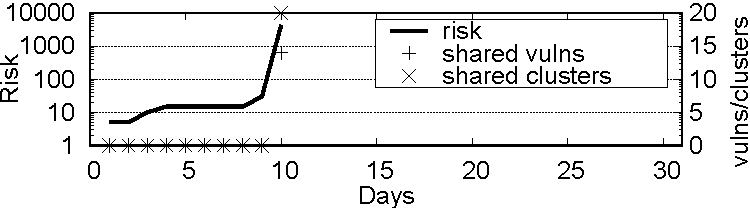
\includegraphics[width=0.5\columnwidth]{images/gnuplot/score/score_random_all.pdf}\label{fig:random_all}}
\hspace{0.5cm}
\subfigure[\system]{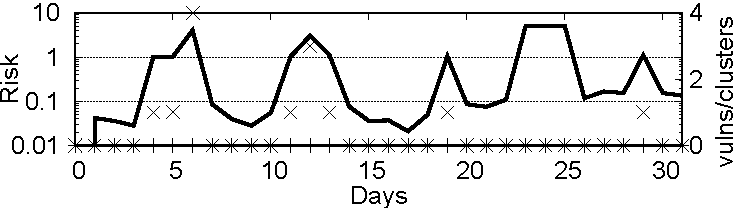
\includegraphics[width=0.5\columnwidth]{images/gnuplot/score/score_final_all.pdf}\label{fig:intel_all}}
\caption{Execution phase for Random and \system OS configuration strategies (log scale).}
\label{fig:run_all}
\end{figure*}

\textbf{Results:} As shown in Figure~\ref{fig:random_all}, \emph{Random} survives only for $10$ days. 
The number of shared clusters and vulnerabilities remains small for the first days. 
Then, there is a replica replacement that adds to the configuration an OS that has common vulnerabilities with the others. 
%Thus, enabling an adversary to compromise enough replicas in the system.

\system survives until the end of the experiment, as the risk is continually managed to keep the system safe. Figure~\ref{fig:intel_all} shows that shared clusters sometimes increase, at the same pace as the risk.
But then, the next reconfigurations are carried out with the goal of decreasing the risk. 
Notice that the risk value is always under $1$ for \system, and in the \emph{Random} is mostly above $10$.


\subsection{Diversity vs Attacks}

\begin{table}[t]
\begin{center}
{%\small%
\footnotesize
\begin{tabular}{ | p{0.96\columnwidth} | }\hline

\textbf{Samba:} 
\emph{On February 2, 2017, security researchers published details about a zero-day vulnerability in Server Message Block (SMB) of Windows, affecting several versions such as 8.1, 10, Server 2012 R2, and Server 2016. 
Could cause a \gls{dos} condition when a client accesses a malicious SMB.}\\
\textbf{CVES:} 
CVE-2017-0016
\\ \hline

\textbf{Wanna Cry:} 
\emph{On Friday, May 12, 2017, the world was alarmed to discover a widespread ransomware attack that hit organizations in more than 100 countries. Based on a vulnerability in Windows' SMB protocol (nicknamed EternalBlue), discovered by the NSA and leaked by Shadow Brokers.} \\
\textbf{CVES:} 
CVE-2017-0143, CVE-2017-0144, CVE-2017-0145, CVE-2017-0146, CVE-2017-0147, CVE-2017-0148 \\ \hline

\textbf{PowerShell:} 
\emph{Security feature bypass vulnerabilities in Device Guard that could allow an attacker to inject malicious code into a Windows PowerShell session.} \\
\textbf{CVES:}
CVE-2017-0219, CVE-2017-0173, CVE-2017-0215, CVE-2017-0216, CVE-2017-0218\\ \hline

\textbf{Stackclash:} 
\emph{In its 2017 malware forecast, SophosLabs warned that attackers would increasingly target Linux. The flaw, discovered by researchers at Qualys, is in the memory management of several operating systems and affects Linux, OpenBSD, NetBSD, FreeBSD and Solaris.}\\
\textbf{CVES:}
CVE-2017-1000365, CVE-2017-1000366, CVE-2017-1000367, CVE-2017-1000369, CVE-2017-1000370, CVE-2017-1000370, CVE-2017-1000371, CVE-2017-1000372, CVE-2017-1000373, CVE-2017-1000374, CVE-2017-1000375, CVE-2017-1000376, CVE-2017-1000379, CVE-2017-1083, CVE-2017-1084, CVE-2017-3629, CVE-2017-3630, CVE-2017-3631\\ \hline

\end{tabular}
}
\caption{Notable attacks during 2017.}
\label{tab:special_vulns}
\end{center}
\end{table}

This experiment evaluates the strategies when facing notable attacks/vulnerabilities that appeared in $2017$. 
Each attack potentially exploits several flaws, some of which affecting different \glspl{os}. 
The attacks were selected by searching the security news sites for high impact problems, most of them related to more than one CVE. 
As some of the \glspl{cve} include applications, we added more vulnerabilities to the database for this purpose.
Table~\ref{tab:special_vulns} lists the attacks and related \glspl{cve}: Samba,\footnote{https://www.secureworks.com/blog/attacking-windows-smb-zero-day-vulnerability} WannaCry,\footnote{https://securityintelligence.com/wannacry-ransomware-spreads-across-the-globe-makes-organizations-wanna-cry-about-microsoft-vulnerability/} Powershell,\footnote{http://blog.talosintelligence.com/2017/06/ms-tuesday.html} and Stackclash.\footnote{https://nakedsecurity.sophos.com/2017/06/20/stack-clash-linux-vulnerability-you-need-to-patch-now/}


Since some of these attacks might have been prepared months before the vulnerabilities are publicly disclosed, we augmented the execution phase to the full six months. 
As before, the strategies are analyzed over $5000$ runs.


\begin{figure}[t]
\begin{center}
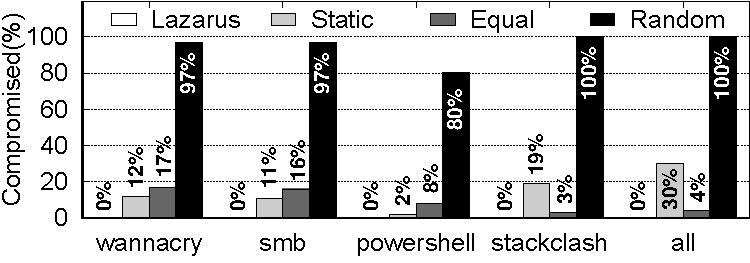
\includegraphics[width=\columnwidth]{images/gnuplot/special_vulns/execution-special.pdf}
\caption{Compromised runs with notable attacks.}
\label{fig:special_vulns}
\end{center}
\end{figure}

\textbf{Results:}
Figure~\ref{fig:special_vulns} shows the percentage of compromised runs for each attack and all attacks put together.
\system is clearly the best at handling the various scenarios, with no compromised executions.
\emph{Random} is the worse, as it does not use any criteria to select the OSes. 
Both \emph{Equal} and \emph{Static} may perform not so bad as they are static, i.e., the \glspl{os} selected by random chance might end up not being exploitable until the end of the run.

\section{Final Remarks}
\label{sec:finalremarkslazarus}

\system addresses the long-standing open problem of evaluating, selecting, and managing the diversity of a \gls{bft} system to make it resilient to malicious adversaries.
Our work focuses on two fundamental issues: how to select the best replicas to run together given the current threat landscape, and what is the performance overhead of running a diverse \gls{bft} system in practice.


\chapter{Supporting Diversity Mechanisms}
\label{chap:supportingdiversitymechanism}
This chapter presents \system iplementation, these mechanisms were implemented to be fully automated, removing the human from the loop.
The current implementation of \system manages 17 \gls{os} versions, supporting the \gls{bft} replication of a set of representative applications.
The replicas run in \glspl{vm}, allowing provisioning mechanisms to configure them. 
We conducted two sets of experiments, one demonstrates that \system risk management can prevent a group of replicas from sharing vulnerabilities over time; the other, reveals the potential negative impact that virtualization and diversity can have on performance. However, we also show that if naive configurations are avoided, \gls{bft} applications in diverse configurations can actually perform close to our homogeneous bare metal setup.
%These results open avenues for many future works in the area. 


\section{\system Implementation}
\label{sec:implementation}

This section details the implementation of each component of \system. 
It also briefly presents other aspects of our prototype.% like the management of replicas running in a virtualized environment.


\subsection{Control Plane}
\label{sec:lazarus}

Figure~\ref{fig:arch1} shows \system control plane with its four main modules, described below.

\begin{figure}[h]
\begin{center}
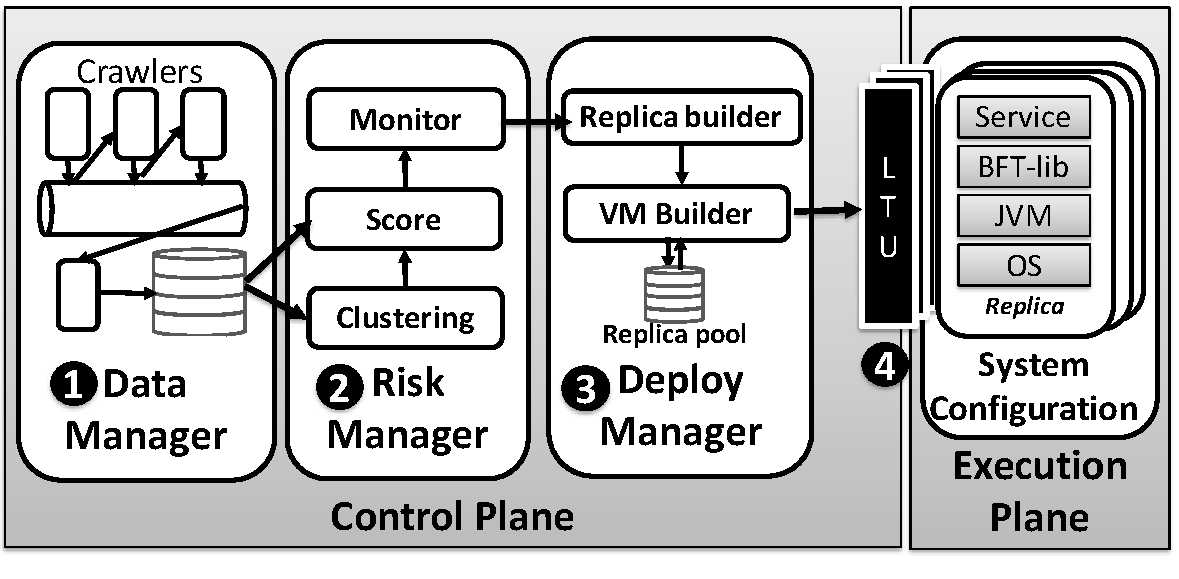
\includegraphics[width=.9\columnwidth]{images/images/architecture_new.pdf}
\vspace{-5mm}
\caption{\system architecture.}
\vspace{-5mm}
\label{fig:arch1}
\end{center}
\end{figure}


\circled{1} \textbf{\fetcher.} \system needs to know the software stack of each available replica to be able to look for vulnerabilities in this software.
The list of software products is provided following the \gls{cpe} Dictionary~\cite{cpe}, which is also used by \gls{nvd}. 
%The \fetcher determines if the CPE list is updated by checking the most recent CPE count in the NVD web page.
For each software, the administrator can indicate the time interval (in years) during which data should be obtained from \gls{nvd}' feeds.

The \fetcher parses the \gls{nvd} feeds considering only the vulnerabilities that affect the chosen products. 
The processing is carried out with several threads cooperatively assemblying as much data as possible about each vulnerability -- a queue is populated with requests pertaining a particular vulnerability, and other threads will look for related data in additional \gls{osint} sources. 
Typically, the other sources are not as well structured as \gls{nvd}, and therefore they have to be handled with specialized HTML parsers that we have developed. 
Currently, the prototype supports five other sources, namely Exploit DB, CVE-details, Ubuntu, Debian, and Microsoft. 
As previously mentioned, such sources provide complementary data, like additional affected products versions not mentioned in \gls{nvd}.

The collected data is stored in a relational database (MySQL).
For each vulnerability we keep its \gls{cve} identifier, the published date, the products it affects, its text description, some \gls{cvss} attributes (e.g., availability and integrity); and exploit and patching dates.


\circled{2} \textbf{\risk.} This component finds out when it is necessary to replace the currently running group of \replicas and discovers an alternative configuration that decreases the risk. 
As explained in Section~\ref{sec:measurerisk}, the risk is computed using score values that require two kinds of data: the information about the vulnerabilities, which is collected by the \fetcher; and the vulnerability clusters. 
A vulnerability cluster is a set of vulnerabilities that are related accordingly to their description (see Section~\ref{sec:details} for details).
The \risk also runs Algorithm~\ref{alg:algorithm2} to monitor the replicated system and trigger reconfigurations.


\circled{3} \textbf{\manager.} 
This component automates the setup and execution of the diverse replicas. 
It creates and deploys the \replicas in the execution environment implementing the decisions of the \risk, i.e., it dictates when and which \replicas leave and join the system. 
We developed a replica builder on top of Vagrant~\cite{vagrant}.
It is responsible for downloading, installing, and configuring the \replicas.
Moreover, it performs replica maintenance, where  \replicas in \QS are booted to carry out automatic software updates (i.e., patching). 


\paragraph{Setup.}
The box configuration is defined in a configuration file, named \emph{Vagrantfile}, consider the example in Listing~\ref{vagrantfile}.
In this file, it is possible to set several options of the box, to name a few:
the box name, the number of CPUs, the amount of memory RAM, the IP, the type of network, sync folders between host and the box, etc. 
Additionally, it is possible to pass some VM-specific parameters, e.g., some CPU/mother board flags such as enabling VT-x technology -- consider the \texttt{modifyvm} fields in Listing~\ref{vagrantfile} (lines 6-14).
It is possible to select different \gls{vm} providers (e.g., libvirt, VMware, VirtualBox, Parallels, Docker, etc), we rely on VirtualBox since it is the one with more diversity opportunities in the Vagrant Cloud~\cite{vagrantcloud}. 
Vagrant Cloud is a website that offers a plethora of different VMs.

\begin{lstlisting}[style=mystyle,caption=Windows Server 2016 Vagrantfile,label=vagrantfile]
Vagrant.configure(2) do |config|
	config.vm.box = "geerlingguy/ubuntu1604"
	config.ssh.insert_key = false
	config.vm.provider "virtualbox" do |v|
		v.customize ["modifyvm", :id, "--cpus", 4]
		v.customize ["modifyvm", :id, "--memory", 22000]
		v.customize ["modifyvm", :id, "--cpuexecutioncap", 100]
		v.customize ["modifyvm", :id, "--ioapic", "on"]
		v.customize ["modifyvm", :id, "--hwvirtex", "on"]
		v.customize ["modifyvm", :id, "--nestedpaging", "on"]
		v.customize ["modifyvm", :id, "--pae", "on"]
		v.customize ["modifyvm", :id, "--natdnshostresolver1", "on"]
		v.customize ["modifyvm", :id, "--natdnsproxy1", "on"]
	end
	config.vm.network "public_network", ip:"192.168.2.50", bridge:"em1"
	config.vm.provision :shell, path: "run_debian.sh", privileged: true
end
\end{lstlisting}

\todo{Add all fields that are mentioned, then add lines to the text}

\paragraph{Download.}
One of the fields of the \emph{Vagranfile} is the boxname, the \texttt{box} field is the key that is used to choose which box will be downloaded, each key is unique for each box.
There are plenty of \glspl{os} and versions ready-to-use, and the same OS/version can have different ``manufacturers" -- some of which are official.

\paragraph{Deploy and provision.}
Vagrant supports complex provisions mechanisms, such as Chef or Puppet, but shell script was sufficient for us. 
This is set in the \emph{Vagranfile} \texttt{provision} field, one can describe the provision steps inline or in an external file and link it to the \emph{Vagranfile}.
Then, when the OS is booting, after the basic setup, the \glspl{os} will execute the provision script.
In this script, we program which software will be downloaded and run in the \glspl{vm} and what configurations are needed. 
We have developed shell scripts for each \glspl{os}, some of which share the same script as Debian and Ubuntu. 
Each \glspl{os}, especially the ones from different \glspl{os} families (e.g., Solaris and BSD) have different commands to execute the same instructions.
Although different, all scripts were meant to do the same thing:
First the script installs the software that is missing in the box -- this is not true for all OSes -- like Java 8, \texttt{wget}, \texttt{unzip}, and any additional software that one wants to install/run after the \glspl{os} boot.



\paragraph{Command and Control.}
There are some simple commands to boot and halt a box, e.g., \texttt{vagrant up} and \texttt{vagrant halt}. 
Vagrant also provides an ssh command (\texttt{vagrant ssh}) that allows the host to connect to the box. 
Our manager component makes the bridge between the \risk and the execution environment.
We developed an API on top of Vagrant, another level of abstraction made to manage replicated systems.


\circled{4} \textbf{LTUs.} Each node that hosts a replica has a Vagrant daemon (see details in next section) running on its trusted domain.
This component is isolated from the internet and communicates only with the \system controller through \gls{tls} channels.

\subsection{Additional Details}
\label{sec:details}

\textbf{Vulnerability Clustering.}
A few steps are carried out to create the vulnerability clusters. 
First, the vulnerability description needs to be transformed into a vector, where a numerical value is associated with the most relevant words (up to 200 words). 
This operation entails, for example, converting all words to a canonical form and calculating their frequency (less frequent words are given higher weights).
Then, the K-means algorithm is applied to build the clusters~\cite{Jain:2010}, where the number of clusters to be formed is determined by the elbow method~\cite{Thorndike:1953}. 
%Currently, it is set $K=200$.
%The algorithm assigns each vulnerability to the cluster with the minimum distance to the cluster center. 
%Then, it computes the cluster centroid, i.e., the average of each data attribute using only the members of a cluster. 
%Next, it calculates the distance of every vulnerability to the centroid, potentially placing them in close clusters. 
%The algorithm stops when there are no further exchanges between clusters.
%We used the elbow method~\cite{Thorndike53whobelongs} to determine the number of clusters to be formed, in our case was $200$ clusters.
We used the open-source machine learning library Weka~\cite{weka} to build the clusters. 


\subsection{Clustering}\label{sec:clustering}
Clustering is the process of aggregating elements into similar groups, named clusters. 
For example, two elements from the same cluster have a higher probability of being similar than two elements from different clusters. 
We apply this technique to build clusters of similar vulnerabilities.
One of the benefits of applying clustering techniques to vulnerability-data is that the algorithm does not need prior knowledge about the data.
It is the process alone that discovers the hidden knowledge in the data.
Each cluster is used as a hint that similar vulnerabilities are likely to be activated through the same or similar exploit.
We considered the vulnerability description and published date to find these similarities. 
In the end, it is expected that the clusters have a minimal number of elements that just represent the same or similar vulnerabilities.


In order to apply a clustering technique to our data, we need to follow some steps:

\paragraph{1) Data representation}
We transform the data that is stored in a database into a format that is readable by the clustering algorithm. 
Since we are using Weka~\cite{weka}, the data must be represented as \gls{arff}. 
Basically, this is a CSV file with some meta information, see Listing~\ref{list:arff}.

\begin{lstlisting}[style=mystyle,caption=ARFF file describing a vulnerability.,label=list:arff]
@RELATION vulnerabilities
@ATTRIBUTE cve string
@ATTRIBUTE description string
@ATTRIBUTE published_date date "yyyy-MM-dd"
@DATA
CVE-2017-3301, 'vulnerability in the solaris component of oracle sun systems products suite subcomponent kernel the supported version that is [...] attacks of this vulnerability can result in unauthorized update insert or delete access to some of solaris accessible data cvss v base score integrity impacts', '2017-01-27'
...more
\end{lstlisting}


This file contains all the vulnerabilities entries in the database. 
As we are interested in the vulnerability similarities, we select only the \gls{cve} identifier, the text, that contains the most relevant and nonstructured information, and the published date.
These attributes add meaning and temporal reference to the clustering algorithm.


\paragraph{2) Data preparation}
In general, machine learning algorithms do not handle raw data, then the data needs to be prepared:
First, we transform the \gls{cve} string into a number, basically, for each \gls{cve}, there is a real number that identifies each \gls{cve} unequivocally. 
This attribute is transformed in numeric values using \emph{StringToNominal} filter. 
Each \gls{cve} identifier is mapped to a numeric value.
Second, we transform the published date to a number format that Weka can handle using the \emph{NumericToNominal} filter.
Third, the text description must be transformed into a vector, the vector will represent the frequencies of each word in the whole document of strings. 
We used the \emph{StringToWordVector} to transform a text string into a vector of word weights, these weights represent the relevance of each word in the document.
This filter contains the following parameters:
\begin{itemize}
\item \textbf{TF- and IDF-Transform}, both set to true, TF-IDF stands for term frequency-inverse document frequency. 
This is a statistical measure used to evaluate how relevant a word is to a document in a collection. 
The relevance increases proportionally to the number of times a word appears in the document but is offset by the frequency of the word in the corpus. 
For example, words that appear in all vulnerability descriptions, are less relevant than the ones that appear more in few vulnerabilities.
\item \textbf{lowerCaseTokens}, convert all the words to lower case.
\item \textbf{minTermFreq}, set to -1, this will preserve any word despite their occurrences in the document.
\item \textbf{normalizeDocLength}, set to normalize all data.
\item \textbf{stopwords}, we define a stop word list, then words from this list are discarded. We begin with a general English stop word list containing pronouns, articles, etc. 
\item \textbf{tokenizer}, set to \emph{WordTokenizer}, this filter will remove special characters from the text, there is a default set of characters but we added a few more.
\item \textbf{wordsTopKeep}, is the number of words that will be kept to make the clusters. We kept $200$ as it was the number of words that represent better the lexical of vulnerabilities after removing the \emph{stopwords}.
\end{itemize}


Our goal is to build clusters in such way that similar vulnerabilities, even if they affect different products, are put together in the same cluster. 
For example, recall the vulnerabilities in Table~\ref{tab:missing_products}, which can be put in the same cluster since they are very similar.
Some of the parameters listed above needed some tuning to achieve our goals.
For example, before the tuning, some of the clusters were representing types of vulnerabilities, e.g., buffer overflow, cross-site scripting, etc. 
Since we are not interested in that type of clusters we have refined our \emph{stopword list} to reduce the description vocabulary to contain only what matters for us.
We have done this by iterating the process and checking the most used words (top 200 words) for clustering (this can be seen in Weka's intermediary output).
Then, we added the most relevant from the 200 words that were deviating from our goal.
In the end, we have a stop word list~\footnote{Stop word list is available: here} without the security-vocabulary noise.


When the pre-filtering ends, Weka presents a file very similar to the previous \gls{arff} file with the difference that the features are the most relevant words in the corpus. And each instance contains a value of relevance for each word.


\paragraph{3) Making clusters}
K-means is an unsupervised machine learning algorithm that groups data in K clusters.
The \emph{K-means} has two important parameters: the number of clusters to be formed, we set to $200$ clusters. We used the elbow method~\cite{Thorndike:1953} to decide $k=200$; and the \emph{distance function}, to calculate the distance between objects, the \emph{Euclidean Distance} is the most adequate for this type of data;
The \emph{K-means} computes the distance from each data entry to the cluster center (randomly selected in the first round).
Then, it assigns each data entry to a cluster based on the minimum distance (i.e., Euclidean distance) to each cluster center.
Then, it computes the centroid, that is the average of each data attribute using only the members of each cluster.
Calculate the distance from each data entry to the recent centroids. 
If there is no modification (i.e., re-arrangement of the elements in the cluster), then the clusters are complete, or it recalculates the distance that best fits the elements. 
When the K-means finishes the execution, we take the cluster assignments of each vulnerability. 
The assignments will be added to a new \gls{arff} file, similar to the first one but with a new attribute that is the cluster name (e.g., cluster1, cluster2, etc). 



Sometimes the resulting clusters include vulnerabilities that are unrelated. Therefore, we use the Jaccard index (J-index) to measure the similarity between the vulnerabilities within the cluster. We calculate the J-index of each element, and then the average J-index of the cluster. 
The clusters with a smaller average J-index (below a certain threshold) are considered ill-formed. In this case, we select the vulnerabilities with lower J-index and move them to another cluster that would result in a better J-index. If no such cluster exists, then we create a new one with the ``orphan'' vulnerability.

\textbf{BFT replication.}
Although there has been relevant research on \gls{bft} protocols over the last twenty years, there are few open-source replication libraries that implement them. \system can use any of those libraries, as long as they support replica set reconfigurations.
More specifically, to manage the \replicas, we need the ability to add first a new \replica to the set and then remove the old \replica to be quarantined. 
Therefore, we employ BFT-SMaRt~\cite{Bessani:2014}, a stable \gls{bft} library that provides reconfigurations on the \replicas set.

\textbf{Replica Virtualization.}
\glspl{vm} can be used to implement replicated systems, leveraging on the isolation between the untrusted and the trusted domains~\cite{Sousa:2010,Platania:2014,Distler:2011}.
Recovery triggering can be initiated from the isolated domain in a synchronous manner, reducing the downtime of the service during the reconfigurations. 
In our implementation, we resort to the Vagrant~\cite{vagrant} provisioning tool to do fast deployment of ready-to-use \glspl{os} and applications on \glspl{vm}. 
Vagrant supports several virtualization providers, e.g., VMware and Docker. 
From the available alternatives, we chose VirtualBox~\cite{virtualbox} because it offers more diversity opportunities, i.e., it supports a more extensive set of different guests \glspl{os}.
%The VMs are available in the Vagrant Cloud~\cite{vagrantcloud}.
\section{Performance Evaluation}
\label{sec:overhead}

In this section, we evaluate how \system' affects the performance of diverse replicated systems.
First, we run the BFT-SMaRt microbenchmarks in our virtualized environment using 17 \gls{os} versions to understand how the performance of a \gls{bft} protocol varies with different \glspl{os}, and how they compare with the performance of a homogeneous bare metal setup.
Second, we use the same benchmarks to measure the performance of specific diverse setups.
Third, we analyze the performance of the system along \system-managed reconfigurations.
Fourth, we measure the time that each OS takes to boot.
Finally, we evaluate the performance of three \gls{bft} services running in the \system infrastructure.


These experiments were conducted in a cluster of Dell PowerEdge R410 machines, where each one has 32 GB of memory and two quad-core 2.27 GHz Intel Xeon E5520 processor with hyper-threading, i.e., supporting 16 hardware threads on each node.
The machines communicate through a gigabit Ethernet network.
Each server runs Ubuntu Linux 14.04 LTS (3.13.0-32-generic Kernel) and VirtualBox 5.1.28, for supporting the execution of VMs with different OSes. 
Additionally, Vagrant 2.0.0 was used as the provisioning tool to automate the deployment process.
In all experiments, we configure BFT-SMaRt v1.1 with four replicas ($f=1$), one replica per physical machine.

Table~\ref{tab:oses} lists the 17 \gls{os} versions used in the experiments and the number of cores used by their corresponding \glspl{vm}.
These values correspond to the maximum number of CPUs supported by VirtualBox with that particular \gls{os}.
The table also shows the \gls{jvm} used in each \gls{os}, and the amount of memory supported by each of these \glspl{vm}.
Given these limitations we setup our environment to establish a fair baseline by configuring an \emph{homogeneous} \gls{bm} environment that uses only four cores of the physical machine. 

%Given the limitations of the VMs we were able to setup in our environment, all experiments conducted in our \emph{homogeneous bare metal environment} (BM) were configured to make BFT-SMaRt replicas use only four cores of the machines, to establish a fair baseline.


\begin{table}[t]
\begin{center}
{\footnotesize
\begin{tabular}{| c | c | c | c | c |}\hline
\textbf{ID} & \textbf{Name}  & \textbf{Cores} & \textbf{JVM} & \textbf{Mem.} \\\hline\hline
UB14 & Ubuntu 14.04 & 4 & Java Oracle 1.8.0\_144 & 15GB \\ \hline
UB16 & Ubuntu 16.04 & 4 & Java Oracle 1.8.0\_144 & 15GB \\ \hline
UB17 & Ubuntu 17.04 & 4 & Java Oracle 1.8.0\_144 & 15GB \\ \hline
OS42 & OpenSuse 42.1 & 4 & Openjdk 1.8.0\_141 & 15GB \\ \hline
FE24 & Fedora 24 & 4 & Openjdk 1.8.0\_141 & 15GB \\ \hline
FE25 & Fedora 25 & 4 & Openjdk 1.8.0\_141 & 15GB \\ \hline
FE26 & Fedora 26 & 4 & Openjdk 1.8.0\_141 & 15GB \\ \hline
DE7 & Debian 7 & 4 & Java Oracle 1.8.0\_151 & 15GB \\ \hline
DE8 & Debian 8 & 4 & Openjdk 1.8.0\_131 & 15GB \\ \hline
W10 & Windows 10 & 4 & Java Oracle 1.8.0\_151 &1GB \\ \hline
WS12 & Win. Server 2012 & 4 & Java Oracle 1.8.0\_151 & 1GB \\ \hline
FB10 & FreeBSD 10 & 4 & Openjdk 1.8.0\_144 & 15GB \\ \hline
FB11 & FreeBSD 11 & 4 & Openjdk 1.8.0\_144 & 15GB \\ \hline
SO10 & Solaris 10 & 1 & Java Oracle 1.8.0\_141 & 15GB \\ \hline
SO11 & Solaris 11 & 1 & Java Oracle 1.8.0\_05 & 15GB \\ \hline
OB60 & OpenBSD 6.0 & 1 & Openjdk 1.8.0\_72 & 1GB \\ \hline
OB61 & OpenBSD 6.1 & 1 & Openjdk 1.8.0\_121 & 1GB \\ \hline
\end{tabular}
}
\caption{The different OSes used in the experiments and the configurations of their VMs and JVMs.}
\label{tab:oses}
\end{center}
\end{table}


\subsection{Homogeneous Replicas Throughput}


We start by running the BFT-SMaRt microbenchmark using the \emph{same \gls{os} version} in all replicas.
The microbenchmark considers an empty service that receives and replies variable size payloads, and is commonly used to evaluate \gls{bft} state-machine replication protocols (e.g., \cite{Castro:1999,Bessani:2014,Liu:2016,Behl:2015,Behl:2017}). 
Here, we consider the $0/0$ and $1024/1024$ workloads, i.e., $0$ and $1024$ bytes requests/response, respectively.
The experiments employ up to 1400 client processes spread on seven machines to create the workload.
% and the throughput was measured in the BFT-SMaRt leader replica.

\textbf{Results:}
Figure~\ref{fig:bftsmart} shows the throughput of each \gls{os} running the benchmark for both loads.
To establish a baseline, we executed the benchmark in our bare metal Ubuntu, without \system virtualization environment.

The results show that there are some significant differences between running the system on top of different \glspl{os}.
This difference is more significant for the $0/0$ workload as it is much more CPU intensive than the $1024/1024$ workload.
Ubuntu, OpenSuse, and Fedora OSes are well supported by our virtualization environment and achieved a throughput around $40k$ and $10k$ for the $0/0$ and $1024/1024$ workloads, which corresponds to approx. $66\%$ and $75\%$ of the bare metal results, respectively.
For Debian, Windows, and FreeBSD, the results are much worse for the CPU intensive $0/0$ workloads but close to the previous group for $1024/1024$.
Finally, single core VMs running Solaris and OpenBSD reached no more than $3000$ ops/sec with both workloads.

These results show that the virtualization platform limitations on supporting different \glspl{os}, strongly limits the performance of specific \glspl{os} in our testbed.

\begin{figure}[h]
\begin{center}
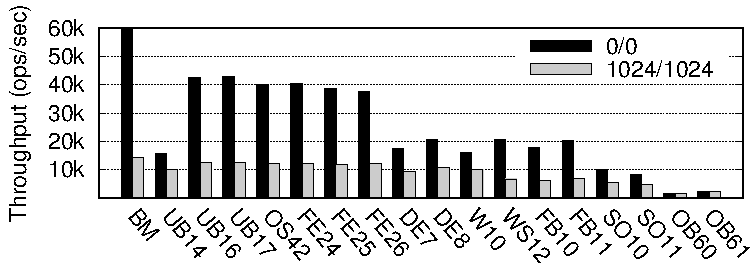
\includegraphics[width=\columnwidth]{images/gnuplot/vagrant/runs_new_new/throughput.pdf}
\caption{Microbenchmark for 0/0 and 1024/1024 (request/replying) for homogeneous OSes configurations.}
\label{fig:bftsmart}
\end{center}
\end{figure}

\subsection{Diverse Replicas Throughput}
\label{sec:performancediversity}

The previous results show the performance of BFT-SMaRt when running on top of different \glspl{os}, but with all replicas running in the same environment.
In this experiment, we evaluate three diverse sets of four replicas, one with the fastest \glspl{os} (UB17, UB16, FE24, and OS42), another with one replica of each \gls{os} family (UB16, W10, SO10, and OB61), and a last one with the slowest \glspl{os} (OB60, OB61, SO10, and SO11).
The idea is to set an upper and lower bound on all possible diverse sets throughput.

\begin{figure}[h]
\begin{center}
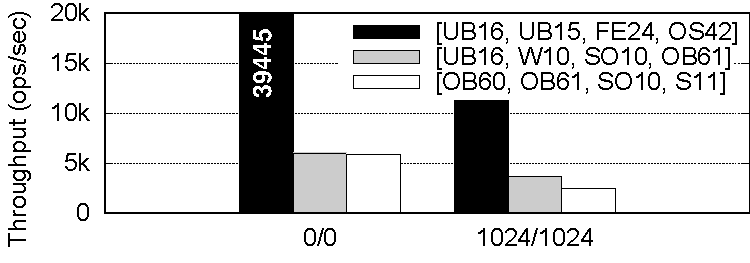
\includegraphics[width=\columnwidth]{images/gnuplot/vagrant/runs_diversity/throughput.pdf}
\caption{Microbenchmark for 0/0 and 1024/1024 (request/reply) for three diverse OS configurations.}
\label{fig:diversets}
\end{center}
\end{figure}


\textbf{Results:}
Figure~\ref{fig:diversets} shows that throughput drops from 39k to 6k for the $0/0$ workload ($65\%$ and $10\%$ of the bare metal performance), and from 11.5k to 2.5k for the $1024/1024$ workload ($82\%$ and $18\%$ of the bare metal performance).
When comparing these two sets with the non-diverse sets of Figure~\ref{fig:bftsmart}, the fastest set is in $7^{th}$, and the slowest set is in $16^{th}$.
It is worth to stress that the slowest set is composed of OSes that only support a single CPU -- due to the VirtualBox limitations -- therefore the low performance is somewhat expected.
The set with \glspl{os} from different families is very close to the slowest set, as two of the replicas use single-CPU \glspl{os}, and BFT-SMaRt always makes progress in the speed of the 3rd fastest replica (a Solaris \gls{vm}), since its Byzantine quorum needs three replicas for ordering requests.
These results show that running \system with current virtualization technology results in a significant performance variation, depending on the configurations selected by the system.
This opens interesting avenues for future work on protocols that consider such performance diversity, as will be discussed in Section~\ref{sec:discussion}.

\subsection{Performance During Reconfiguration}
\label{sec:reconfiguration}



In this experiment, we show how \system-triggered reconfigurations affect the replicas' performance.
Reconfigurations, in this case, subsumes to the addition of a new replica and the removal of the old one, using the BFT-SMaRt reconfiguration protocols~\cite{Bessani2014}. 
We execute this experiment with an in-memory \gls{kvs} service that comes with the BFT-SMaRT library.
%This service mimics the basic ``BFT Zookeeper'' application benchmark shown in recent BFT papers~\cite{Liu16,Behl:2017}.

The experiment was conducted with a \gls{ycsb}~\cite{Cooper:2010} workload of $50\%$ of reads and $50\%$ of writes, with values of 1024 bytes associated with small numeric keys, varying the state size of the \gls{kvs}.
We run this experiment for $400$ seconds, and reconfigure the set of replicas with a period of $100$ seconds. 
The initial \gls{os} configuration is the fastest OS set (i.e., UB17, UB16, FE24, OS42).
\begin{figure}[h]
\subfigure[KVS state size $\approx 30$MBs.]{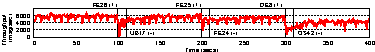
\includegraphics[width=\textwidth]{images/gnuplot/vagrant/reconfiguration/reconfiguration_state10mbs.pdf}\label{fig:s10mbs}}
\subfigure[KVS state size $\approx 60$MBs.]{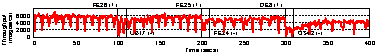
\includegraphics[width=\textwidth]{images/gnuplot/vagrant/reconfiguration/reconfiguration_state50mbs.pdf}\label{fig:s50mbs}}
\caption{KVS performance with \system-triggered reconfigurations on a 50/50 YCSB workload and 1kB-values.}
\label{fig:reconfiguration}
\end{figure}



\textbf{Results:}
Figure~\ref{fig:reconfiguration} shows two types of performance drops.
The first type happens at every 1000 writes and is due to the state checkpoints used to trim the operation logs.
The second type is more severe and less frequent, and happens during reconfigurations, mostly due to the state transfer to the new replica joining the system.
These types of performance perturbations, which become more severe with bigger states, were already identified, and mitigated in previous works~\cite{Bessani:2013}.\footnote{We employ the standard checkpoint and state transfer protocols of BFT-SMaRt and not the one introduced in~\cite{Bessani:2013} as the developers of the system pointed them as more stable.} 

The figure shows that the reconfigurations take around $10$ seconds for these setups, and did not change significantly with states of approx. $30$ and $60$ MBs.
Regarding diversity, the figure shows no noticeable disruption when changing Ubuntu 17 to Fedora 26 and Fedora 25 to Fedora 24, but the replacement of a Debian 8 by an OpenSuse 42 replica significantly decreases the performance, which is consistent with the results from Figure~\ref{fig:bftsmart}.

\subsection{Booting time}

Before triggering a reconfiguration, \system needs to start the new \gls{vm}, boot the \glspl{os}, and launch the BFT-SMaRt replica.
Therefore, the total time to replace a ``risky'' replica roughly comprises the time required to boot the new OS plus the reconfiguration time (discussed in the previous section).
This experiment measures the boot time of the \glspl{os} supported by \system prototype. 

\begin{figure}[h]
\begin{center}
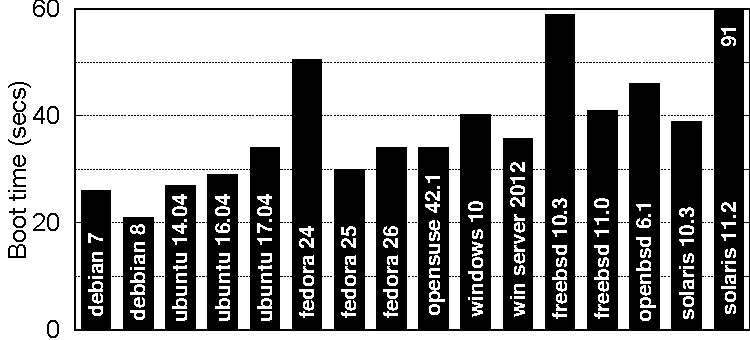
\includegraphics[width=.8\columnwidth]{images/gnuplot/vagrant/updown/boot.pdf}
\vspace{-5mm}
\caption{OSes boot times (seconds).}
\label{fig:boot}
\end{center}
\end{figure}

\textbf{Results:}
Figure~\ref{fig:boot} shows the average boot time of $20$ executions boot for each \gls{os}.
As can be seen, most \glspl{os} take less than 40s to boot, with exceptions of Fedora 24 (50s), FreeBSD 10.3 (59s), and Solaris 11.2 (91s).
In any case, these results together with the reconfiguration times of the previous section show that \system can react to a new threat in less than two minutes (in the worst case).

\subsection{Application Benchmarks}
Our last set of experiments aims to measure the throughput of three existing \gls{bft} services built on top of BFT-SMaRt when running in \system.
The considered applications and workloads are:

\begin{itemize}

\item \emph{KVS} is the same BFT-SMaRt application employed in Section~\ref{sec:reconfiguration}.
It represents a consistent non-relational database that stores data in memory, similarly to a coordination service (an evaluation scenario used in many recent papers on \gls{bft}~\cite{Liu:2016,Behl:2017}).
In this evaluation, we employ the \gls{ycsb} $50\%/50\%$ read/write workload with values of 4k bytes.

\item \sieveq~\cite{Garcia:2016} is a \gls{bft} message queue service that can also be used as an application-level firewall, filtering messages that do not comply with a pre-configured security policy.
Its architecture, based on several filtering layers, reduces the costs of filtering invalid messages in a BFT-replicated state machine.
In our evaluation, we consider all the layers were running on the same four physical machines as the diverse BFT-SMaRt replicas (under different OSes).
The workload imposed to the system is composed of messages of 1k bytes.

\item \emph{BFT ordering for Hyperledger Fabric}~\cite{Sousa:2018} is the first \gls{bft} ordering service for Fabric~\cite{Androulaki:2018}. 
Fabric is an extensible blockchain platform designed for business applications beyond the basic digital coin.
The ordering service is the core of Fabric, being responsible for ordering and grouping issued transactions in signed blocks that form the blockchain.
In our evaluation, we consider transactions of 1k bytes, blocks of $10$ transactions and a single block receiver.

\end{itemize}

As in Section~\ref{sec:performancediversity}, we run the applications on the fastest and slowest diverse replica sets and compare them with the results obtained in bare metal.

\textbf{Results:}
Figure~\ref{fig:apps} shows the peak sustained throughput of the applications. 
The \gls{kvs} results show a throughput of 6.1k and 1.2k ops/sec, for the fastest and slowest configurations, respectively.
This corresponds to $86\%$ and $18\%$ of the 7.1k ops/sec achieved on bare metal.

The \sieveq results show a smaller performance loss when compared with bare metal results.
More specifically, \sieveq in the fastest replica set reaches $94\%$ of the throughput achieved on the bare metal.
Even with the slowest set, the system achieved $53\%$ of the throughput of bare metal.
This smaller loss happens due to the layered architecture of \sieveq, in which most of the message validations happen before the message reaches the \gls{bft} replicated state machine (which is the only layer managed by \system).

The Fabric ordering service results show that running the application on \system virtualization infrastructure lead to $91\%$ (fastest set) to $39\%$ (slowest set) of the throughput achieved on bare metal. 

Nonetheless, even the slowest configurations would not be a significant bottleneck if one takes into consideration the current performance of Fabric~\cite{Sousa:2018}
%Overall, the relatively poor results for the slowest set are due to the single-core and low-memory setups of their replicas (see Table~\ref{tab:oses}).

\begin{figure}[t]
\begin{center}
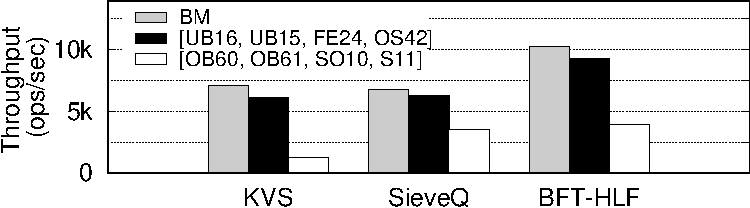
\includegraphics[width=\columnwidth]{images/gnuplot/vagrant/runs_apps/throughput.pdf}
\vspace{-5mm}
\caption{Different BFT applications running in the bare metal, fastest and slowest OS configurations.}
\vspace{-3mm}
\label{fig:apps}
\end{center}
\end{figure}



\section{Final Remarks}
\label{sec:finalremarkslazarus}

\system addresses the long-standing open problem of evaluating, selecting, and managing the diversity of a \gls{bft} system to make it resilient to malicious adversaries.
Our work focuses on two fundamental issues: how to select the best replicas to run together given the current threat landscape, and what is the performance overhead of running a diverse \gls{bft} system in practice.


\chapter{Untrusted (distributed) controller}
\label{chap:controler}

As in previous works~\cite{Roeder:2010,Platania:2014}, our current design for \sieveq and \system considers a centralized trusted control plane that analyze \gls{osint} and orchestrate replica group reconfigurations.
It would be desirable to have a distributed version of such control plane, not only for improving its dependability, but also to support the existence of multi-domain applications, such as blockchain platforms.


%\chapter{\sieveq Evaluation}
\label{chap:sieveqevaluation}




%\chapter{\system Evaluation}
\label{chap:lazarusevaluation}


\section{Evaluation of Replica Set Risk}
\label{sec:diversity}

This section evaluates how \system performs on the selection of dependable \replica configurations.
As discussed in Section~\ref{sec:replica}, we focus our experimental evaluation solely on the OS diversity.
% These play a crucial role in any IT system, and most of the \replica's code is the OS. 
% Thus, they present a high potential to become the most vulnerable part of a \replica.
% Hence, in the following experiments, we explore OS diversity among the replicas. 

In these experiments, we emulate live executions of the system by dividing the collected data into two periods:
(i) a \emph{learning phase} covering all vulnerability data between \emph{2010-1-1} and \emph{2017-9-29}, which is used to setup the \risk's algorithm; and (ii) an \emph{execution phase} composed of the period between \emph{2017-10-1} and \emph{2018-3-30}.
This last period is divided into three intervals of two months (OUT-NOV, DEC-JAN, and FEB-MAR), allowing for three independent tests.
%JAN-FEB, MAR-APR, and MAY-JUN
The goal is to create a knowledge base in the \emph{learning phase} that is used to assess \system choices during each interval of the \emph{execution phase}. 
A run starts on the first day of an interval and then progresses through each day of the interval until the end. Every day, we check if the currently executing replica set could be compromised by an attack exploring the vulnerabilities released on that day. 
We take the most pessimist approach, which is to say that we consider the system to be broken if a vulnerability comes out that affects at least two OSes that would be executing at that time.

Three additional strategies, inspired by previous works, were defined to be compared with \system (Section~\ref{sec:configurations}):

\begin{itemize}
\item \textbf{Equal:} all the replicas use the same randomly-selected OS during the whole execution. 
This strategy corresponds to the scenario where most past \gls{bft} systems have been implemented and evaluated (e.g.,~\cite{Kotla:2010,Aublin:2015,Behl:2015,Veronese:2013,Behl:2017,Liu:2016,Yin:2003,Amir:2011,Bessani:2014,Clement:2009b}). 
Here, compromising a replica would mean an opportunity to intrude the remaining ones.

\item \textbf{Static:} a configuration of $n$ different \glspl{os} is randomly selected, and there are no changes during the whole execution. 
This corresponds to a diverse \gls{bft} system without reconfigurations (e.g.,~\cite{Rodrigues:2001}).

\item \textbf{Random:} a configuration of $n$ \glspl{os} is randomly selected, and at the beginning of each day, a new \gls{os} is randomly picked to replace an existing one. 
This solution represents a system with proactive recovery and diversity, but with no informed strategy for choosing the next \configuration.

%\item \textbf{\system}, $n$ OSes are chosen based the algorithm described in Section~\ref{sec:measurerisk}. This algorithm decides when it is time to replace OSes, which OS is out and which OS is in.
\end{itemize}

The experiments consider a pool of 38 \gls{os} versions to be deployed on four replicas. 
At the beginning of the execution phase, the OSes are assumed to be fully patched.

%\begin{figure}[t]
%\begin{center}
%\includegraphics[width=\columnwidth]{figs/gnuplot/executions/execution.pdf}
%\caption{Compromised system runs over 2 month slots.}
%\label{fig:all_vulns}
%\end{center}
%\end{figure}



\subsection{Diversity vs Vulnerabilities}
We evaluate how each strategy can prevent the replicated system from being compromised. 
Each strategy is analyzed over $5000$ runs throughout the execution phase in two-month slots. 
Different runs are initiated with distinct random number generator seeds, resulting in potentially different \gls{os} selections over the time slot. 
On each day, we check if there is a vulnerability affecting more than one replica in the current \configuration, and in the affirmative case the execution is stopped.

\begin{figure}[h]
\begin{center}
\includegraphics[width=\columnwidth]{images/gnuplot/executions_new/execution.pdf}
\caption{Compromised system runs over 2 month slots.}
\label{fig:all_vulns}
\end{center}
\end{figure}

\textbf{Results:} Figure~\ref{fig:all_vulns} compares the percentage of compromised runs of all strategies. 
Each bar represents the percentage of runs that did not terminate successfully (lower is better). 
In all three periods, \system presents the best results. 
The \emph{Random} strategy performs worse because eventually, it picks a group of \glspl{os} with common vulnerabilities. 
This result provides evidence for the claim that \system improves the dependability, reducing the probability that $f+1$ \glspl{os} eventually become compromised. 
Interestingly, and contrary to intuition, changing \glspl{os} every day with no criteria will always create unsafe configurations.
Therefore, it is paramount to have selection strategies like the ones we use in \system.
\note{Add all the months we already have}

\subsection{Risk evaluation}


In order to better understand how \system performed, we isolated one of the $5000$ runs to observe the risk evolution over time. 
We picked the \emph{Random} and \system strategies for this analysis, with results displayed in Figure~\ref{fig:run_all}. 
The graphs present the evolution of the common vulnerabilities, the common clusters, and our risk metric for both schemes. 
Notice that two \glspl{os} might appear in the same cluster but with no mutual flaw as clusters can include many distinct vulnerabilities.

\begin{figure*}[h]
\subfigure[Random]{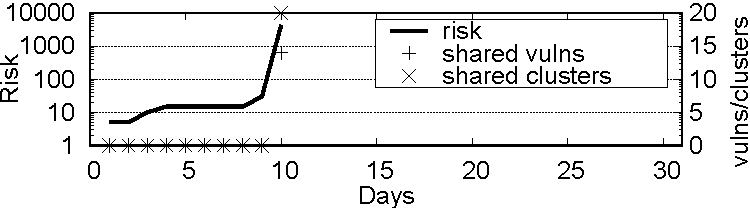
\includegraphics[width=0.5\columnwidth]{images/gnuplot/score/score_random_all.pdf}\label{fig:random_all}}
\hspace{0.5cm}
\subfigure[\system]{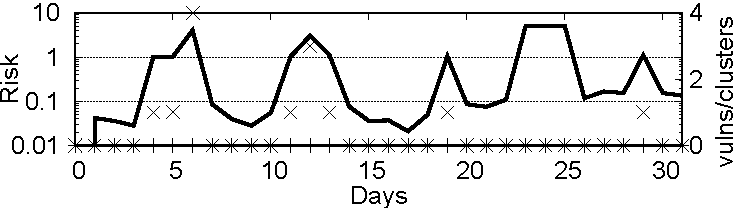
\includegraphics[width=0.5\columnwidth]{images/gnuplot/score/score_final_all.pdf}\label{fig:intel_all}}
\caption{Execution phase for Random and \system OS configuration strategies (log scale).}
\label{fig:run_all}
\end{figure*}

\textbf{Results:} As shown in Figure~\ref{fig:random_all}, \emph{Random} survives only for $10$ days. 
The number of shared clusters and vulnerabilities remains small for the first days. 
Then, there is a replica replacement that adds to the configuration an OS that has common vulnerabilities with the others. 
%Thus, enabling an adversary to compromise enough replicas in the system.

\system survives until the end of the experiment, as the risk is continually managed to keep the system safe. Figure~\ref{fig:intel_all} shows that shared clusters sometimes increase, at the same pace as the risk.
But then, the next reconfigurations are carried out with the goal of decreasing the risk. 
Notice that the risk value is always under $1$ for \system, and in the \emph{Random} is mostly above $10$.


\subsection{Diversity vs Attacks}

\begin{table}[t]
\begin{center}
{%\small%
\footnotesize
\begin{tabular}{ | p{0.96\columnwidth} | }\hline

\textbf{Samba:} 
\emph{On February 2, 2017, security researchers published details about a zero-day vulnerability in Server Message Block (SMB) of Windows, affecting several versions such as 8.1, 10, Server 2012 R2, and Server 2016. 
Could cause a \gls{dos} condition when a client accesses a malicious SMB.}\\
\textbf{CVES:} 
CVE-2017-0016
\\ \hline

\textbf{Wanna Cry:} 
\emph{On Friday, May 12, 2017, the world was alarmed to discover a widespread ransomware attack that hit organizations in more than 100 countries. Based on a vulnerability in Windows' SMB protocol (nicknamed EternalBlue), discovered by the NSA and leaked by Shadow Brokers.} \\
\textbf{CVES:} 
CVE-2017-0143, CVE-2017-0144, CVE-2017-0145, CVE-2017-0146, CVE-2017-0147, CVE-2017-0148 \\ \hline

\textbf{PowerShell:} 
\emph{Security feature bypass vulnerabilities in Device Guard that could allow an attacker to inject malicious code into a Windows PowerShell session.} \\
\textbf{CVES:}
CVE-2017-0219, CVE-2017-0173, CVE-2017-0215, CVE-2017-0216, CVE-2017-0218\\ \hline

\textbf{Stackclash:} 
\emph{In its 2017 malware forecast, SophosLabs warned that attackers would increasingly target Linux. The flaw, discovered by researchers at Qualys, is in the memory management of several operating systems and affects Linux, OpenBSD, NetBSD, FreeBSD and Solaris.}\\
\textbf{CVES:}
CVE-2017-1000365, CVE-2017-1000366, CVE-2017-1000367, CVE-2017-1000369, CVE-2017-1000370, CVE-2017-1000370, CVE-2017-1000371, CVE-2017-1000372, CVE-2017-1000373, CVE-2017-1000374, CVE-2017-1000375, CVE-2017-1000376, CVE-2017-1000379, CVE-2017-1083, CVE-2017-1084, CVE-2017-3629, CVE-2017-3630, CVE-2017-3631\\ \hline

\end{tabular}
}
\caption{Notable attacks during 2017.}
\label{tab:special_vulns}
\end{center}
\end{table}

This experiment evaluates the strategies when facing notable attacks/vulnerabilities that appeared in $2017$. 
Each attack potentially exploits several flaws, some of which affecting different \glspl{os}. 
The attacks were selected by searching the security news sites for high impact problems, most of them related to more than one CVE. 
As some of the \glspl{cve} include applications, we added more vulnerabilities to the database for this purpose.
Table~\ref{tab:special_vulns} lists the attacks and related \glspl{cve}: Samba,\footnote{https://www.secureworks.com/blog/attacking-windows-smb-zero-day-vulnerability} WannaCry,\footnote{https://securityintelligence.com/wannacry-ransomware-spreads-across-the-globe-makes-organizations-wanna-cry-about-microsoft-vulnerability/} Powershell,\footnote{http://blog.talosintelligence.com/2017/06/ms-tuesday.html} and Stackclash.\footnote{https://nakedsecurity.sophos.com/2017/06/20/stack-clash-linux-vulnerability-you-need-to-patch-now/}


Since some of these attacks might have been prepared months before the vulnerabilities are publicly disclosed, we augmented the execution phase to the full six months. 
As before, the strategies are analyzed over $5000$ runs.


\begin{figure}[t]
\begin{center}
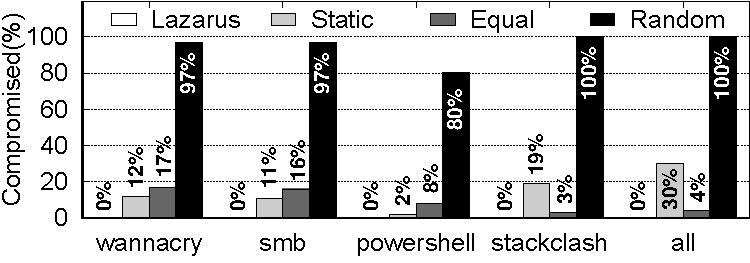
\includegraphics[width=\columnwidth]{images/gnuplot/special_vulns/execution-special.pdf}
\caption{Compromised runs with notable attacks.}
\label{fig:special_vulns}
\end{center}
\end{figure}

\textbf{Results:}
Figure~\ref{fig:special_vulns} shows the percentage of compromised runs for each attack and all attacks put together.
\system is clearly the best at handling the various scenarios, with no compromised executions.
\emph{Random} is the worse, as it does not use any criteria to select the OSes. 
Both \emph{Equal} and \emph{Static} may perform not so bad as they are static, i.e., the \glspl{os} selected by random chance might end up not being exploitable until the end of the run.


\section{Discussion}
\label{sec:discussionlazarus}

\chapter{Conclusion and Future Research Directions}
\label{chap:conclusion}

\section{Summary of the Results}
\system addresses the long-standing open problem of evaluating, selecting, and managing the diversity of a BFT system to make it resilient to malicious adversaries.
Our work focuses on two fundamental issues: how to select the best replicas to run together given the current threat landscape, and what is the performance overhead of running a diverse BFT system in practice.
Our results open many avenues for future work on this topic.

\paragraph{OS vulnerability Study}
The main results could be summarized as follows:
\begin{enumerate}
\item In most diverse \gls{os} configurations, significant  benefits in security could be observed: a low number of vulnerabilities were found to affect more than one \gls{os};

\item The number of vulnerabilities that affect more than one \gls{os} depends on how diverse the configuration is: they are higher for OSes from the same family (e.g., BSD) but very low (and in many cases zero) in OSes from different families (e.g., BSD and Windows);

\item We presented several strategies for system designers to choose most diverse \glspl{os} using \gls{nvd} data depending on whether they: consider all common vulnerabilities as being of equal importance; place greater emphasis on more recent common vulnerabilities (and hence wish to minimise the number of those); are primarily interested in the common vulnerabilities being reported less frequently in calendar time (which would allow them more time to respond to them). Surprisingly, for our dataset, all three strategies delivered the same best combination of four \glspl{os} for an intrusion-tolerant configuration (four being the usual number of systems needed to tolerate a Byzantine failure in a replicated system), which is: \textit{\{OpenBSD, Debian, Solaris, Windows2003\}}.

\end{enumerate}



\section{Future Work}

\textbf{Pretest replicas:}
Run a battery of tests (like Fuzzing, vulnerability detectors etc) before the system is running.

\textbf{Use vulnerable clone decttors on Opens source software to aggravete pairs with more clones} with dependcy graphs and autidting tools~\cite{Kim:2017}

\textbf{Test diversity agains automatic attacks, sometimes it may not be perfact, as the attacks we expect to see are APTs, however the idea is to verify if it takes more time to attack a replicated system with diversity}~\cite{Hu:2015}

\textbf{Vulnreabilities in the black market as a inditicar of severity}~\cite{Allodi:2014}.

\textbf{Virtualization technology:}
\system paid a performance penalty due to the limitations of the virtualization platform we used (VirtualBox).
VirtualBox was selected because it was the platform we could run more OSes.
Therefore its use enabled \system to support 17 different OSes for running BFT systems.
It would be great to have a VM technology capable of supporting all existing OSes without the resource limitations we experienced.

\textbf{Distributed control plane:}
As in previous works~\cite{Roeder:2010,Platania:2014}, our current design for \system considers a centralized trusted control plane that analyzes OSINT and orchestrates replica set reconfigurations.
It would be desirable to have a distributed version of such control plane, not only for improving its dependability but also to support the existence of multi-domain applications, such as blockchain platforms.

\textbf{Trusted components:}
Our prototype implements the LTU as a trusted component isolated from the rest of the replica in a VM, as many works on hybrid BFT~\cite{Veronese:2013,Roeder:2010,Platania:2014,Sousa:2010,Distler:2011}.
The recent popularization of trusted computing technologies such as Intel SGX~\cite{sgx}, and its use for implementing efficient BFT replication~\cite{Behl:2017}, open interesting possibilities for using novel hardware to support services like \system on bare metal.

\textbf{Integration with other sensors:}
\system monitors only five security data feeds on the internet looking for vulnerabilities, exploits, and patches in the OSes it manages, but it could be extended to monitor other indicators of compromise (e.g., IP black lists) extracted from a much richer set of sources~\cite{Liao:2016,Sabottke:2015}.
Similarly, \system can be extended to additionally use the outputs of IDSes to assess the BFT system behavior and trigger replica reconfigurations in case of need.

\textbf{Diversity-aware replication:}
The evaluation of BFT-SMaRt on top of \system shows that different replica set configurations can impact on the performance of applications, mostly due to the performance heterogeneity of the different OSes.
It would be interesting to consider protocols in which this heterogeneity is taken into account.
For example, the leader could be allocated in the fastest replica, or weighted-replication protocols such as WHEAT~\cite{Sousa:2015} could be used to assign higher weights to the replicas running in faster replicas.




% Fim do conteudo
% ----------------------------------------------------------------------

% Glossario

%
% Para actualizar o glossario, e' preciso correr o script ./fazindice
% e voltar a gerar o PDF
%
\LIMPA
\renewcommand{\glossaryname}{Acronyms}

\newacronym{aslr}{ASLR}{Address Space Layout Randomization}
\newacronym{arff}{ARFF}{Attribute-Relation File Format}
\newacronym{apts}{APTs}{Advanced Persistent Threats}



\newacronym{bft}{BFT}{Byzantine Fault Tolerance}
\newacronym{bm}{BM}{Bare Metal}

\newacronym[plural=CVEs,firstplural=Common Vulnerabilities and Exposures (CVEs)]{cve}{CVE}{Common Vulnerabilities and Exposures}
\newacronym{cpe}{CPE}{Common Platform Enumeration}
\newacronym{cvi}{CVI}{Common Vulnerability Indicator}
\newacronym{cvcs}{CVCst}{Common Vulnerability Count Strategy}
\newacronym{cvc}{CVC}{Common Vulnerability Count}
\newacronym{cvis}{CVIst}{Common Vulnerability Indicator Strategy}
\newacronym{irt}{IRT}{Inter-Reporting Times}
\newacronym{irts}{IRTst}{Inter-Reporting Times Strategy}
\newacronym{ip}{IP}{Internet Protocol}

\newacronym[plural=GPUs,firstplural=Graphics Processing Units (GPUs)]{gpu}{GPU}{Graphics Processing Unit}
\newacronym[plural=FPGAs,firstplural=Field-Programmable Gate Arrays (FPGAs)]{fpga}{FPGA}{Field-Programmable Gate Array}


\newacronym{cvss}{CVSS}{Common Vulnerability Scoring System}
\newacronym{xss}{XSS}{Cross-site scripting}


\newacronym{cots}{COTS}{Components Off-the-Shelf}
\newacronym{cis}{CIS}{CRUTIAL Information Switch}
\newacronym{dos}{DoS}{Denial-of-Service}
\newacronym{ddos}{DDoS}{Distributed Denial-of-Service}
\newacronym{dbms}{DBMS}{Databases Management Systems}
\newacronym{dns}{DNS}{Domain Name System}

\newacronym[plural=DBs,firstplural=Databases (DBs)]{db}{DB}{Database}

\newacronym{hmac}{HMAC}{Hash-based Message Authentication Code}


\newacronym{jvm}{JVM}{Java Virtual Machine}
\newacronym{ics}{ICS}{Industrial Control Systems}

\newacronym{ots}{OTS}{Off-the-Shelf}
\newacronym{osi}{OSI}{Open Systems Interconnection}

\newacronym[plural=OSes,firstplural=Operating Systems (OSes)]{os}{OS}{Operating System}
\newacronym[plural=IDSs,firstplural=Intrusion Detection Systems (IDSs)]{ids}{IDS}{Intrusion Detection System}


\newacronym{sql}{SQL}{Structured Query Language}

\newacronym[plural=MACs,firstplural=Message Authentication Codes (MACs)]{mac}{MAC}{Message Authentication Code}

\newacronym{nist}{NIST}{National Institute of Standards and Technology}
\newacronym{nvd}{NVD}{National Vulnerability Database}
\newacronym{nfs}{NFS}{Network File System}


\newacronym{ltu}{LTU}{Logical Trusted Unit}

\newacronym{scada}{SCADA}{Supervisory Control and Data Acquisition}
\newacronym{smr}{SMR}{State Machine Replication}
\newacronym{siem}{SIEM}{Security Information and Event Management}

\newacronym{udp}{UDP}{User Datagram Protocol}

\newacronym{ycsb}{YCSB}{Yahoo! Cloud Serving Benchmark}



\newacronym{osint}{OSINT}{Open Source Intelligence}
\newacronym{osvdb}{OSVDB}{Open Sourced Vulnerability Database}

\newacronym{tom}{TOM}{Total Ordered Multicast}
\newacronym{tls}{TLS}{Transport Layer Security}


\newacronym{mtd}{MTD}{Moving Target Defense}


\newacronym{po}{PO}{Proactive Obfuscation}

\newacronym{pr}{PR}{Proactive Recovery}
\newacronym{prr}{PRR}{Proactive-Reactive Recovery}
\newacronym{prrw}{PRRW}{Proactive-Reactive Recovery Wormhole}

\newacronym{zda}{ZDA}{Zero-Day Attack}
\newacronym{pzda}{PZDA}{Pseudo Zero-Day Attack}
\newacronym{ppzda}{PPZDA}{Potential Pseudo Zero-Day Attack}
\newacronym{poa}{POA}{Potential for Attack}


\newacronym{rsa}{RSA}{Rivest–Shamir–Adleman}
\newacronym{kvs}{KVS}{Key-Value Storage}
\newacronym{kmp}{KMP}{Knuth–Morris–Pratt}


\newacronym{svm}{SVM}{Support Vector Machines}
\newacronym{scit}{SCIT}{Self-Cleaning Intrusion Tolerance}

\newacronym{sha}{SHA}{Secure Hash Algorithm }

\newacronym{tcp}{TCP}{Transmission Control Protocol}
\newacronym{wine}{WINE}{Worldlwide Intelligence Network Environmnet}


\newacronym[plural=VMs,firstplural=Virtual Machines (VMs)]{vm}{VM}{Virtual Machine}
\newacronym{vmm}{VMM}{Virtual Machine Manager}
\newacronym{vpn}{VPN}{Virtual Private Network}

\newacronym{xml}{XML}{Extensible Markup Language}




\printglossaries
\addcontentsline {toc} {chapter} {Acronyms}
% Bibliografia

\LIMPA
\bibliographystyle{abbrv}
\bibliography{chapters/references/references}
\addcontentsline {toc} {chapter} {Bibliography}

\end{document}
